\documentclass[oneside,masters,bibliography=totoc]{CooperEE}
  \usepackage[pdftex]{graphicx}
  \usepackage{subcaption}
  \title{Detection of Maliciously Authored News Articles}
  

\usepackage{fancyhdr}

\fancyfoot[C]{{\textbf{\thepage}}}
\pagestyle{fancy}


\fancypagestyle{plain}{
    \fancyhf{}
    \renewcommand{\headrulewidth}{0pt}
    \cfoot{\textbf{\thepage}}
}


\renewcommand{\chaptermark}[1]{ \markboth{}{\thechapter.  #1} } % Add Chapter # and chapter title to header -- should only add it if section mark isnt already there

\renewcommand{\sectionmark}[1]{\markright{\thesection \ \ #1}}

\usepackage[margin=0.3in,labelfont=bf,labelsep=none]{caption}
 \DeclareCaptionFormat{suggested}{\singlespace#1#2 #3\par\doublespace}
 \captionsetup{format=suggested}

\usepackage{cite}

\usepackage{makeidx}
\makeindex


% Make proper left and right quotes
\usepackage [english]{babel}
\usepackage [autostyle, english = american]{csquotes}
\MakeOuterQuote{"}

% ------------------------- 
\Month{December} \Day{11} \Year{2017}
\Author{Miraj Patel}

\TitleTop{Detection of Maliciously}
\TitleBottom{Authored News Articles}
\Advisor{Dr. Carl Sable}
\Dean{Dr. Richard J. Stock}
\DeanTitle{Dean, School of Engineering}
\ThesisDefenseDate{12/11/2017}

\usepackage[bookmarksnumbered,pdfpagelabels=true,plainpages=false,
            colorlinks=true,linkcolor=black,citecolor=black,urlcolor=blue,
            pdfauthor={Miraj Patel},
            pdftitle={Fake News Classification}]
            {hyperref}
% ------------------------- 


\Abstract{
   The 2016 U.S. presidential campaigns were rocked by various scandals, many of which were ignited by fake news articles that spread like wildfire on social media platforms like Facebook and Twitter.  When it came to light that many of these articles were purposefully constructed by foreign actors to influence the presidential election, it became apparent that social media platforms needed more safeguards to prevent individuals from deceiving the public for personal gain.
   
   This study attempts to fulfill this need by building an automated system capable of detecting the malicious content published during the 2016 presidential campaign season.  Using a set of articles flagged as false by Snopes, and a set of articles from leading news organizations, select machine learning algorithms (k-nearest neighbors, support vector machines, and long short-term memory networks) are trained using only each article's textual content.  Other instances of these models are also given the sentiment-related features of each article to take advantage of any possible correlation between the overall sentiment of an article and its factual accuracy.  The results of this study show that a long short-term memory network is capable of obtaining an overall accuracy and average F1-score of 90\% with this dataset.
}

\Acknowledgments{
   First and foremost, I want to thank my advisor Carl Sable.  It was a great privilege to learn from him throughout my undergraduate and graduate careers at Cooper Union.  Without Dr. Sable's guidance and mentorship, this thesis would certainly not have been possible.
   
   I would also like to thank Cooper Union, and the Cooper Union community, for providing me with scholarships to pursue higher learning in these great halls.  I would also like to thank the Electrical Engineering Department and all the professors that have I have had the privilege to learn from throughout my academic career.
   
   I also want to thank Matthew Gentzkow and Chuan Yu for sharing their findings and shaping part of the dataset used in this study.   Lastly, I want to thank my friends and family who supported me throughout this journey.
}

\usepackage{titlesec}
% Make the Chapter #: Chapter Name on same line
\titleformat{\chapter}[hang] 
{\normalfont\huge\bfseries}{\chaptertitlename\ \thechapter:}{1em}{} 
% Decrease the padding between chapter titles
\titlespacing*{\chapter}{0pt}{-50pt}{40pt}



%\usepackage{hyperref}
\PassOptionsToPackage{hyphens}{url}\usepackage{hyperref}
\hypersetup{
colorlinks=true,
breaklinks=true,
%linkcolor=black,
urlcolor=black}

\hypersetup{breaklinks=true}
\urlstyle{same}


\begin{document}

% ------------------------- 
% no need to modify
 \frontmatter
 \makepreliminarypages
 \singlespace
 \tableofcontents
 \clearemptydoublepage
 \listoffigures
 \clearemptydoublepage
 \doublespace
 \mainmatter
% ------------------------- 

%For a file this big, you're better off using the \input command for individual chapters: http://www.tac.dk/cgi-bin/info2www?(latex)\input
\chapter{Introduction}

The practice of producing false narratives and spreading lies to influence the masses was seen as early as 1279 B.C.E. when Ramesses II told his people that his first major excursion, only 5 years into his reign as pharaoh, against the Hittites was a resounding success.  However, the reality was that he had barely managed to make it home alive after being duped by Hittite spies and losing a large majority of his army in his first battle.  As the head of the totalitarian government of Egypt, Ramesses II was able to literally etch his false narrative into stone in an effort to convince his subjects he was superior to their enemies and would build a legacy greater than the pharaohs before him \cite{weir}.  Even some of America's greatest heroes are guilty of deceiving the public to sway public opinion, such as Benjamin Franklin who falsely portrayed Native Americans as murderous scalping enthusiasts, working with King George III, in order to rile up revolutionaries and gain the French's support in the American Revolution \cite{politicoHistoryOfFakeNews}.

Modern technology and higher literacy rates have made it possible for more people to understand the world around them; thus, much of the modern populace can now freely form their own opinions rather than faithfully accept whatever they are told.  The impact of unchecked social media proliferation has led to a new surge of information sharing by established and freelance journalists, small digital publications, large media conglomerates, and inexperienced, yet opinionated and influential, individuals who had previously never shown an interest in public service of any kind.  Recent estimates show that over 67\% of Americans get at least some of their news from social media \cite{pewNewsAcrossSocialMedia}.  The influx of unregulated media vying for Americans' attention makes it difficult to determine whether or not the sources of information Americans now turn to are even legitimate, let alone accurate.  Furthermore, the mounting pressure many journalists face to meet urgent deadlines or publish alerts and updates quickly, in as little as 15 minutes, may make verifying a story for accuracy exceedingly difficult \cite{breakingNewsDrill}.

However, the scenario that unfolded during the United States' 2016 presidential campaign season had little to do with journalists failing to do their due diligence.  By many accounts, fake news, or stories "[intended] to deceive, often geared towards getting clicks", spread through social media platforms like Facebook and Twitter, enwrapping millions of Americans and influencing their perception of the leading contenders in the presidential race \cite{fakeNewsDef}.  In fact, the FBI, along with other American intelligence agencies, concluded that the Russian government was the real author of some of the most trending fake news, including "pizzagate" \cite{newsweekSputnik}.  More recently, British Prime Minister Theresa May publicly denounced Russia for undermining the West's free society by "weaponizing information" and "deploying [Russia's] state-run media organizations to plant fake stories" \cite{englandFakeNews}.  Similarly, Spain accused Russia for employing similar tactics to divide the Spanish people with disinformation \cite{cataloniaFakeNews}.  Thus, the threat posed by maliciously written articles still looms on many parts of the web and could impact upcoming democratic elections.

This study seeks to lay the foundations for developing an autonomous system capable of filtering out untrustworthy content, such as the material that was spread on social media by Russian bots \cite{russianBots}.  One property of a successful system would be the ability to filter out deceitful content written by repeat offenders.  For example, Paul Horner, one of the most prolific fake news authors, composed his work just to showcase how gullible the public was \cite{fakeNewsAuthor}.  In the past, forensic linguists have shown that analysis of idiolects, individuals' distinctive use of language, can help to positively identify anonymous authors, like James Madison as the author of some disputed Federalist Papers, and Ted Kaczynski as the Unabomber and author behind the terrorist manifesto titled \textit{An Industrial Society and Its Future} \cite{federalistPapers, forensicLinguistics}.  To that effect, this study aims to train classifiers that can use not only article content, but also the hidden markers indicative of authors that aim to deceive their readers.

Chapter 2 of this thesis discusses the select algorithms and techniques that are ultimately used in this study.  Afterwards, an overview of the current state of the art in discerning fact from fiction is provided in Chapter 3.  Next, the results of the various experiments using machine learning are presented in Chapter 4.  Finally, this study is concluded in Chapter 5 with an analysis of its successes and shortcomings.



\chapter{Background}

Feature and classifier selection are both crucial for classification using machine learning; analyzing the key properties of a dataset with the model best suited for that domain tends to lead to better results.  Classical machine learning classifiers require numerical values to represent observations of each class.  Since the datasets in natural language processing (NLP) tasks are usually raw text, as is the case for this research study, there must be a conscientious choice on how to accurately portray the text numerically.  Two NLP techniques to produce vectorized representations of text documents are presented in this chapter: term frequency-inverse document frequency score weighting, and word embeddings.  This chapter also includes a section on preprocessing techniques to refine the textual data, as well as a brief synopsis on the field of sentiment analysis to motivate the idea that sentiment scores can be important features for this study since they provide insight about the motivation and purpose of a piece of text.  Lastly, this chapter formally introduces the classifier models used in this research: k-nearest neighbors, support vector machines, and recurrent neural networks.


\section{Preprocessing} \label{preprocessingSection}
Real-world data is usually messy.  One of the first steps before performing any data analysis is to clean or refine the data by making the data structured and correct, and removing any discernible noise.  The preprocessing steps performed in this study fall into the category Jurafsky and Martin call "text normalization" because the text is being converted into a convenient and standard form \cite{preprocessing}.  The very first step in text processing is to tokenize the data, or separate the words.  Though common practice is to simply use whitespace and punctuation to delimit words, compound words such as proper nouns (e.g., "White House") can lose their meaning when broken up.  To overcome this information loss, named entity recognizers can be used to prevent splitting up these tokens.

To standardize the data, the tokens may then be converted to their roots so different tenses of words can be linked together.  However, this task, called lemmatization, requires that the words in each sentence are first tagged with their part-of-speech to determine the root word.  Since part-of-speech tagging is sometimes too computationally intensive for large documents, a simpler approach called stemming is often used in its place.  Stemming aims to remove the suffixes of each word to get the root.  However, the effectiveness of the stemmer is implementation dependent.  For example, the Porter stemmer aims to remove suffixes using pattern matching, potentially producing incoherent words or semantically incorrect words (e.g., the stem of "ties" is "ti", and the stem of "operator" is "operate") \cite{porterStemmer}.  Finally, to refine the text of the document, articles, pronouns, prepositions, and other uninformative words are sometimes filtered out before the core analysis is performed.  These uninformative words, called stop words, usually help in information retrieval and document similarity tasks \cite{stopWord}.


\section{Term Frequency-Inverse Document Frequency} \label{tfidfSection}

Once preprocessing is complete, the remaining text must be transformed into real-valued vectors so that the text can be used by a model.  One technique to produce numerical values for words in a document is to represent each word by its term frequency-inverse document frequency score.  The term frequency-inverse document frequency (tf-idf) of a word is used to quantify the importance of a word in a corpus based on how frequently the word shows up in a document and how many other documents also contain the word \cite{tfidf}.

\begin{equation}
\label{eq:tfidf}
\mbox{tf-idf}_{w,d_{i},D} = ( \frac{c_{w}}{|d_{i}|} ) \cdot \log ( \frac{|D|}{1 + |d  \in  D : w  \in  d|} ) 
\end{equation}

A basic tf-idf scoring function is available in Eq. \ref{eq:tfidf}.  The first term represents the term frequency (tf) of the word $w$, which is the ratio of the number of occurrences of the word ($c_{w}$) to the total number of words in the document ($|d_{i}|$).  The second term is the inverse document frequency (idf) which serves to boost rarer, more informative words, and diminish the impact of frequently used non-informative words, like articles and pronouns.  Since the idf is computed by taking the logarithm of the total number of documents in the corpus ($|D|$) divided by the number of documents with the word offset by 1 to avoid 0 denominators ($1 + |d  \in  D : w  \in  d|$), words that appear in almost all the documents will have a idf close to 0.  On the other hand, words that appear in only select documents will have larger idf values, thereby increasing their tf-idf weights.

\section{Word Embeddings}

\begin{figure}[h]
\centering
\captionsetup{justification=centering,width=0.95\textwidth}
\centerline{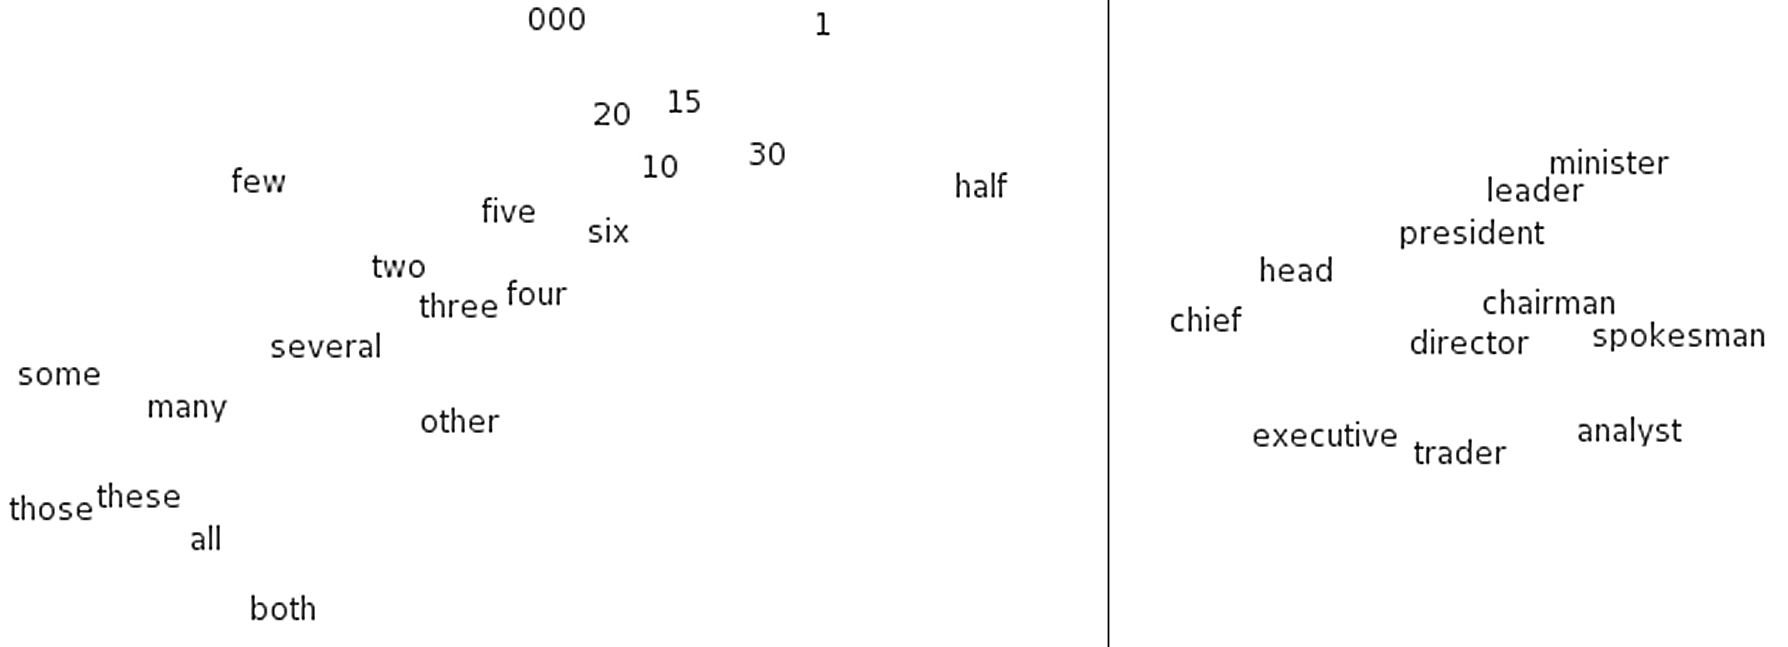
\includegraphics[width=0.95\textwidth]{similarWordVectors.png}}
\caption[t-SNE Visual of Numbers and Occupations]{
    t-SNE visualization of word embeddings \cite{wordEmbeddingImg}\\
    Left: the number region in a word embedding model\\
    Right: the occupations region
}
\label{fig:similarWordVectors}
\end{figure}


Another way to numerically represent a text is to use a word embedding model to transform each word into a real-valued vector.  The word embedding of a word is the high-dimensional vector that is the result of mapping the word with a parameterized function that was developed using a large corpus that is representative of the source language.  One of the primary benefits of using word embeddings is that similar words will tend to map to the same region.  t-distributed stochastic neighbor embedding (t-SNE) is a probabilistic technique designed for dimensionality reduction, and can be used to visualize high-dimensional datasets like word embeddings \cite{tsneAbout}.  The t-SNE algorithm converts similarities between data points into joint probabilities and tries to minimize the divergence between these joint probabilities and the high-dimensional data \cite{tsneVisual, tsnePython}.  Due to the reduction in dimensionality, mainly for the purposes of visualization, the axes and its units on t-SNE plots do not have any real meaning; however, the t-SNE still meaningfully shows which of the points are closer together in the original feature space \cite{tsneAxes}.  An example of the benefit is shown in Fig. \ref{fig:similarWordVectors} which shows zoomed-in views on the number and jobs regions of a t-SNE visual constructed using word embeddings.


\begin{figure}[h]
\centering
\captionsetup{justification=centering,width=0.95\textwidth}
\centerline{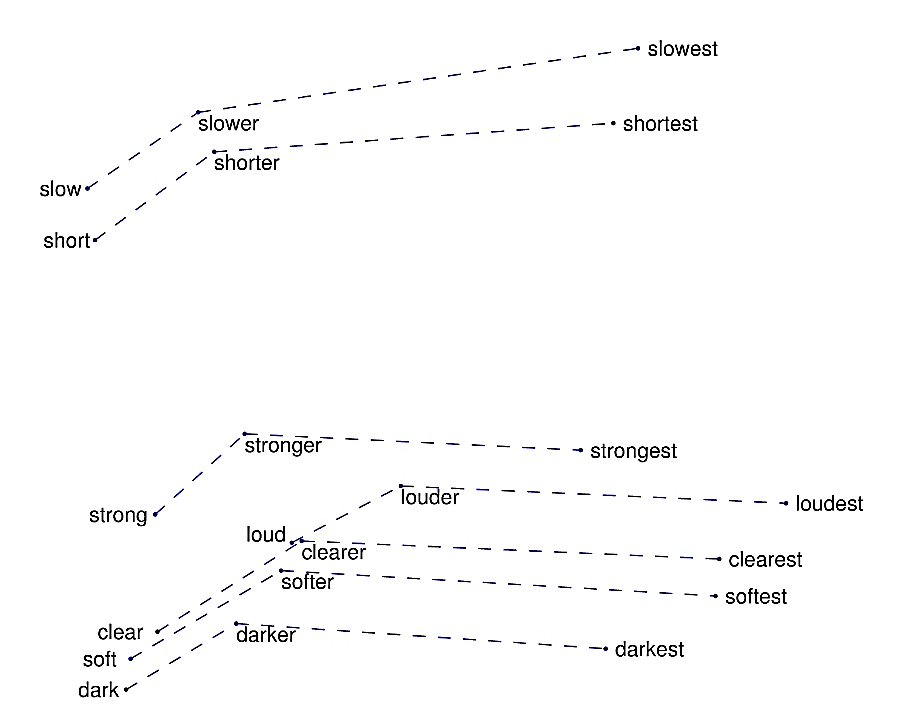
\includegraphics[width=0.65\textwidth]{comparativeVsSuperlative.png}}
\caption[t-SNE Visual of Comparative and Superlative Words]{
    t-SNE visual of GloVe word embeddings for select comparative and superlative words \cite{comparativeVsSuperlative}
}
\label{fig:comparativeVsSuperlative}
\end{figure}


The word embedding model used in this study is the GloVe model that was trained by a team of Stanford researchers using global word-to-word co-occurrence statistics.  This vector representation model proves to be highly effective at grouping together similar or related words in higher dimensions.  Furthermore, the model was designed in way such that vector differences between two words' word embeddings capture "the meaning specified by the juxtaposition of two words" \cite{glove}.  For example, the conceptual difference between "short", "shorter", and "shortest" is similar to the difference between "slow", "slower", and "slowest".  Using the underlying words' GloVe word embedding vectors, this conceptual difference is mirrored by vector differences in the t-SNE plot in Fig. \ref{fig:comparativeVsSuperlative}.


\section{Sentiment Analysis} \label{sentimentAnalysisSection}

One common text categorization task is sentiment analysis, which is the identification of sentiment-related features such as the author's positive or negative orientation towards the subject of the text.  Closely related is opinion mining which relates to the extraction and analysis of opinion about entities.  In most literature, and in this paper, the two terms are used interchangeably since the two tasks have become synonymous with each other \cite{sentimentApp}.  Texts such as movie, book, or product reviews, are clear examples of authors expressing their opinions, and sentiments, towards the product.  Similarly, editorials and political texts express the author's sentiment toward the political candidate or the political action that is the subject of the text \cite{nbSentiment}.

Sentiment analysis can be performed at varying granularities: document-level, sentence-level, and aspect-level.  As the terminology hints, document- and sentence-level sentiment analysis aim to classify the sentiment of the text using the whole document as a singular unit.  By classifying constituent sentences, a heuristic can be applied using these lower-level results.  On the other hand, aspect-level sentiment analysis aims to classify sentiment with respect to particular entities, such as parts of a products or distinct characteristics of a person \cite{sentimentApp}.

The potential, and observed, applications of sentiment analysis include product opinion gathering and monitoring, bias detection, automated recommendation engines, and even question answering and automated summarization \cite{sentimentAnalysis}.  Tasks such as product reception, review analysis, and suggesting other products to users based on their reviews are textbook examples of document- and sentence-level sentiment analysis.  Effective question answering systems need to be able to discern the aspect with which questions are asked; that is, whether not the question is purely fact-oriented, or is inherently opinionated and, thus, seeks an opinion-oriented response.  Similarly, summarization benefits from understanding the viewpoints of the text to provide a more cohesive output.


\section{$K$-Nearest Neighbors} \label{knnSection}

The $k$-nearest neighbors (KNN) algorithm is a decision-boundary based classification algorithm that classifies an input to the majority class of its $k$ nearest neighbors in space \cite{knnIR}.  The tunable hyperparameters for this algorithm include $k$, the number of neighbors used for classifying any given input, and the distance metric used for determining the closest neighbors.  The least robust KNN is thought to be $k$ = 1 because this model runs the risk of becoming heavily reliant on noise or outliers.  Variants of KNN may weigh the votes of training set observations with their cosine similarity relative to their input, as shown in Eq. \ref{eq:knnClassScore}.

\begin{equation}
\label{eq:knnClassScore}
score(c, d) = \sum_{d' \in S_{k}(d)} (I_{c}(d') \cdot cos(v(d'), v(d))
\end{equation}

In this scoring weighting scheme, $S_{k}(d)$ is the set of $d$'s $k$ nearest neighbors and $I_{c}(d')$ is the indicator function which equals 1 if and only if the observation $d'$ is part of class $c$, otherwise 0 \cite{knnIR}.

The advantages of KNN as a classification algorithm for practical applications are numerous.  As a non-parametric learning algorithm, KNN requires no assumption on the underlying distribution of the input data.  For applications in natural language processing, specifically classification of news articles as genuine or maliciously authored for political gain, there is not enough substantial evidence to map the articles' text to a closed form probabilistic distribution.  Furthermore, since KNN is an instance-based algorithm, the only "learning" required is to load the observations into memory, which significantly reduces training time \cite{knnGuide}.

As with any machine learning algorithm, KNN also has some drawbacks.  Testing inputs with KNN requires all of the training set to be in memory, or available through some highly performant data store, like a database, so vectorized inputs can be compared with every training point to determine the $k$ nearest neighbors.   However, because our dataset is not too large, this limitation is not a burden for our task.  Another downside to KNN is the time cost for testing: for each individual input, every training point must be checked to see if it is one of the $k$ nearest neighbors, and if so, use its label for classification.  As it turns out, even this limitation does not severely impact testing performance due to the size of the dataset; thus, a trained KNN model is highly performant and can be used for real-time classification \cite{knnGuide}.


\section{Support Vector Machines} \label{svmSection}

The support vector machine (SVM) classifier is a high performing machine learning algorithm that relies on the relatively simple concept of dividing the data into distinct regions.  For example, in binary classification, SVMs seek to maximize the distance between the data points of opposing classes and the dividing decision boundary.   The decision boundary, also known as the hyperplane, is formulated as a linear combination of weights on each dimension of the input, as shown in Eq. \ref{eq:hyperplane}.  $w$ is the vector of weights applied to input $x$, a support vector, whose length corresponds to the dimensionality of $x$, and $b$ is the bias, a constant offset.


\begin{equation}
\label{eq:hyperplane}
w^{T}x + b = 0
\end{equation}


The data points closest to the hyperplane are called the support vectors, and the shortest distance between these points and the boundary is called the margin.  By maximizing the margin, the probability for misclassification due to noise is reduced, assuming that the testing data points come from the same distribution as the training data.  One clear advantage of using SVMs is the low memory cost: only these support vectors need to be held in memory; the other data points, which are farther away from the hyperplane, no longer need to be considered (recall that the KNN algorithm requires every input be compared with every training observation to determine the most likely class) \cite{svmIR}.  

However, in most practical applications, the data cannot directly be separated into 2 well-defined regions, especially for complex datasets with a lot of overlap in the original feature space.  In these instances, it may be possible to map the feature space into a higher dimension where the classes are more easily separable.  However, this mapping may be too complex and computationally intensive to apply to large training sets \cite{svmTutorial}.  This computational complexity can be avoided altogether by using symmetric kernel functions on the pair of vectors, which results in a similarity score that is exactly equivalent to the dot product of its inputs when mapped into a higher dimensional space without having to explicitly map the vectors and computing their dot product, as shown in Eq. \ref{eq:kernelSubstitution} \cite{bishop}.


\begin{equation}
\label{eq:kernelSubstitution}
K(x, x') = \phi(x)^{T}*\phi(x') = \phi(x')^{T}*\phi(x) = K(x', x)
\end{equation}


One example use-case for this higher-order mapping is when the classes' data points are radially dependent.  As shown in Fig. \ref{fig:radialSeparation}, the data can be mapped to $R^{3}$ using the mapping function in Eq. \ref{eq:r3Mapping}.


\begin{equation}
\label{eq:r3Mapping}
z^{2} = x^{2} + y^{2}
\end{equation}


\begin{figure}[h]
\centering
\captionsetup{justification=centering,width=0.95\textwidth}
\centerline{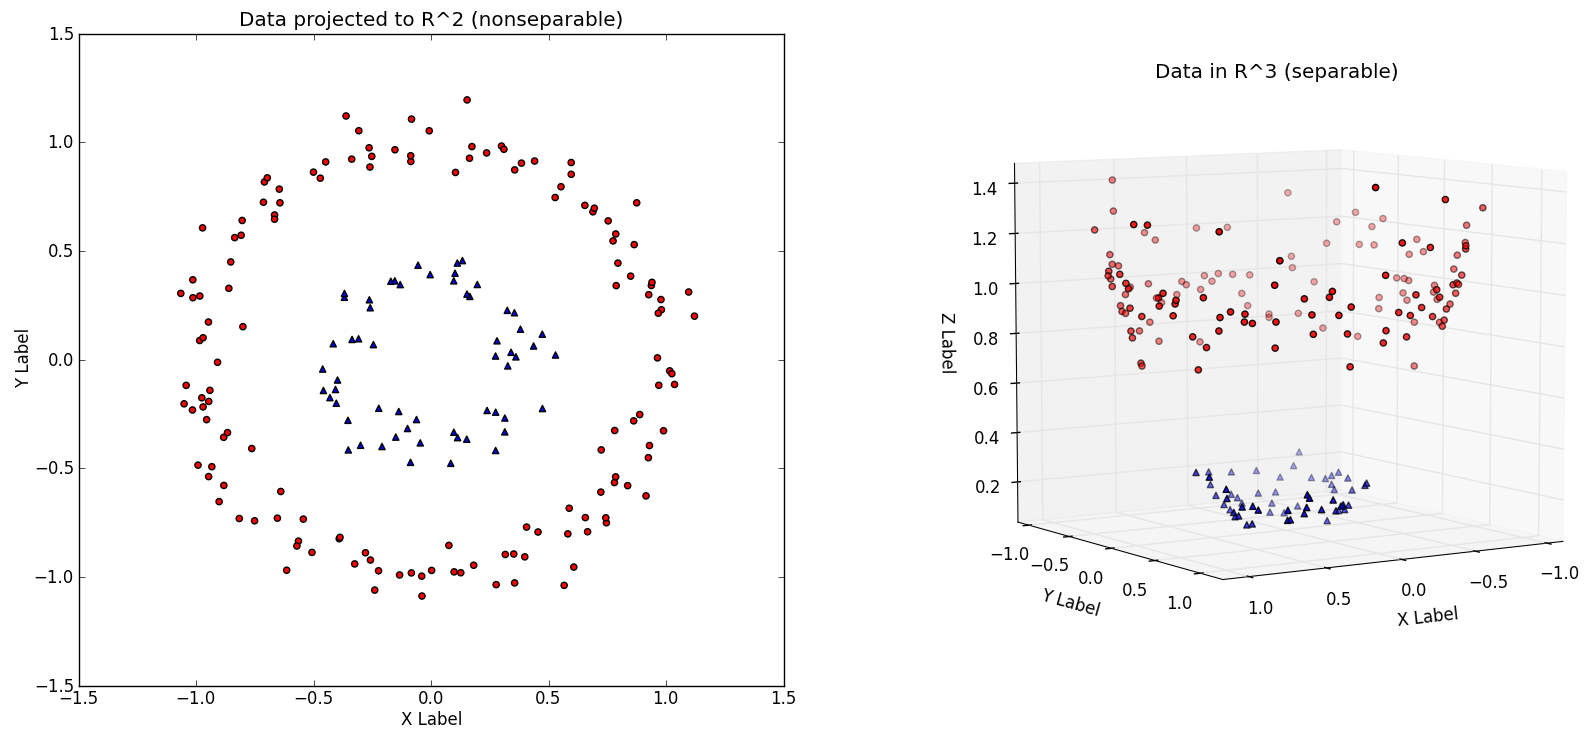
\includegraphics[width=0.95\textwidth]{radialSeparation.png}}
\caption[Mapping Observations from Radially Dependent Classes]{
    Visualizing 2-dimensional observations from two radially dependent distributions \cite{radialSeparation}\\
    Left: 2-D plot of the dataset where $x$ is the X-Label and $y$ is the Y-Label\\
    Right: Dataset is mapped into $R^{3}$ where $z$ is the radius from the origin
}
\label{fig:radialSeparation}
\end{figure}


The analogous radial basis function (RBF) kernel, also known as the Gaussian kernel, is show in Eq. \ref{eq:rbfEq} \cite{rbfKernel}:


\begin{equation} \label{eq:rbfEq}
K(x, x') = exp(-\gamma \cdot ||x-x'||^{2})
\end{equation}


\section{Neural Networks} \label{nnSection}

One of the most popular models that can be found in a modern-day machine learning engineer's toolkit is a neural network.  Though they are at the forefront of many modern  advances and innovations in artificial intelligence, they are far from new.  The idea of an artificial neuron dates as far back to 1943 when McCulloch and Pitts used their knowledge of neurology to devise their mathematical neuron that emulated simple neurons that acted in a binary fashion by firing when the sum of their inputs surpassed some internal threshold \cite{mccullochPitts}.  This simple neuron from 1943 is the foundation for the basic unit now known as a perceptron: a node with various inputs that are summed together to produce a binary result.  A perceptron (shown in Fig. \ref{fig:perceptron}) on its own is the simplest, single-layer neural network, and the weighted sum of its inputs models a linear classifier that can be used for binary classification.  In fact, the optimal values for each weight is learned during training just as the weights and bias are learned for a linear classifier.


\begin{figure}[h]
\centering
\captionsetup{justification=centering,width=0.95\textwidth}
\centerline{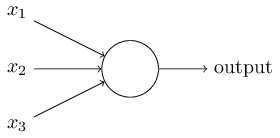
\includegraphics[width=0.65\textwidth]{perceptron.png}}
\caption[Perceptron Model] {
    A perceptron with three inputs: $x_{1}, x_{2}, x_{3}$ \cite{perceptron}
}
\label{fig:perceptron}
\end{figure}


Another key parameter when training a perceptron is its activation function, the input dependent function that decides whether or not the perceptron fires, that is, whether its output is 0 or 1.  In fact, if the simple perceptron emulates a linear classifier with the form in Eq. \ref{eq:hyperplane}, the perceptron's activation function is the Heaviside function (aka step function) since it classifies input vectors as class 0 on negative values and class 1 on positive values.  This classifier is also known as the simplest artificial neural network (ANN or NN) because it is a single layer of perceptrons: the weighted inputs are fed directly to the outputs.  To build more a complex model capable of making more complex decisions, layers of perceptrons are combined to create a network of nodes.  Such networks have historically been called multi-layer perceptrons (MLPs), even though modern networks are usually composed of neurons with other activation functions like the sigmoid, tanh, and rectified linear unit (ReLU) functions, which are shown in Fig. \ref{fig:activationFn} \cite{neuralNetsNLP}.


\begin{figure}[h]
\centering
\captionsetup{justification=centering,width=0.95\textwidth}
\centerline{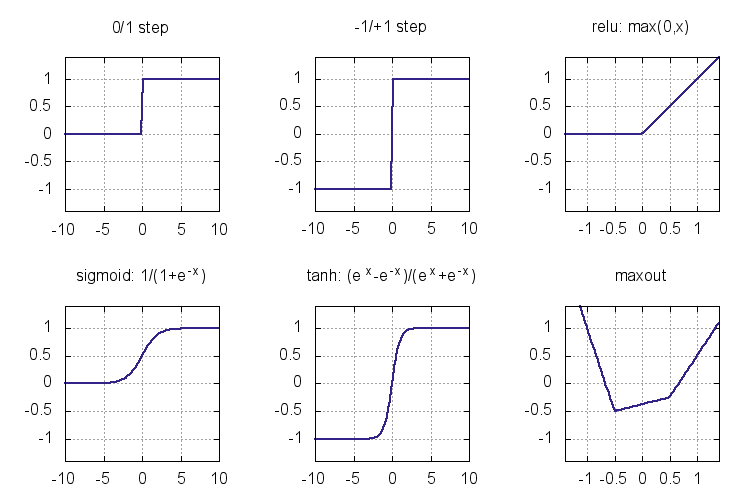
\includegraphics[width=0.95\textwidth]{activationFn.png}}
\caption[Activation Functions]{
    Common activation functions for artificial neurons \cite{activationFn}
}
\label{fig:activationFn}
\end{figure}


The layers that provide the interface between the input and output nodes are called hidden layers.  In typical feedforward networks, the layers of the network are fully connected, and unidirectional.  Thus, the information is strictly moving forward from the input towards the output and there are no cycles or loops.  Typical training of neural networks involves choosing the optimal architecture for the application, which in turn implies choosing the number of hidden layers, and number of nodes in each hidden layer.  The weights of the links between nodes are usually initialized to random values, and then trained with a technique called backpropagation.  Using the chosen loss function that penalizes misclassifications, the delta, or the difference between the model output and true value, of each training iteration is propagated backwards through the network to incrementally update the weights in order to minimize the loss function.  The learning rate of the model dictates at what pace the weights will follow the direction of the delta.  High learning rates will cause the model to take large steps in the direction of the delta, possibly overshooting the minimum and requiring extra iterations; on the other hand, smaller learning rates may lead to slower or incomplete training since many more iterations may be required to reach the minimum loss \cite{neuralNetsNLP}.


\section{Recurrent Neural Networks} \label{rnnSection}

Another class of neural networks showing great promise in the NLP domain is the recurrent network.  In contrast to feedforward networks, recurrent neural networks (RNNs) have directed cycles.  The primary advantage that cycles provide to RNNs is the ability to "[remember] information about what has been calculated so far" since each internal state is dependent on all of the previous computations and states leading up that state \cite{introRNN}.

The cycle in the RNN also allows the RNN to continuously transition between internal states for the entire length of the input sequence.  Thus, while basic feedforward neural networks have strict dimensional requirements for their input and output vectors, RNNs are able to dynamically operate on sequences of vectors \cite{rnn}.  For example, if the input sequence is a sentence with 5 words, the unrolled network would have 5 layers.  Fig. \ref{fig:rnnUnrolled} shows an RNN that unfolds into t+1 layers, where each layer (\textbf{A}) represents an internal state that was computed using the previous state and the next available piece of the input sequence (\textbf{x\textsubscript{t}}).  Note that an activation function can also be applied at each internal state to produce an output (\textbf{h\textsubscript{t}}).


\begin{figure}[h]
\centering
\captionsetup{justification=centering,width=0.95\textwidth}
\centerline{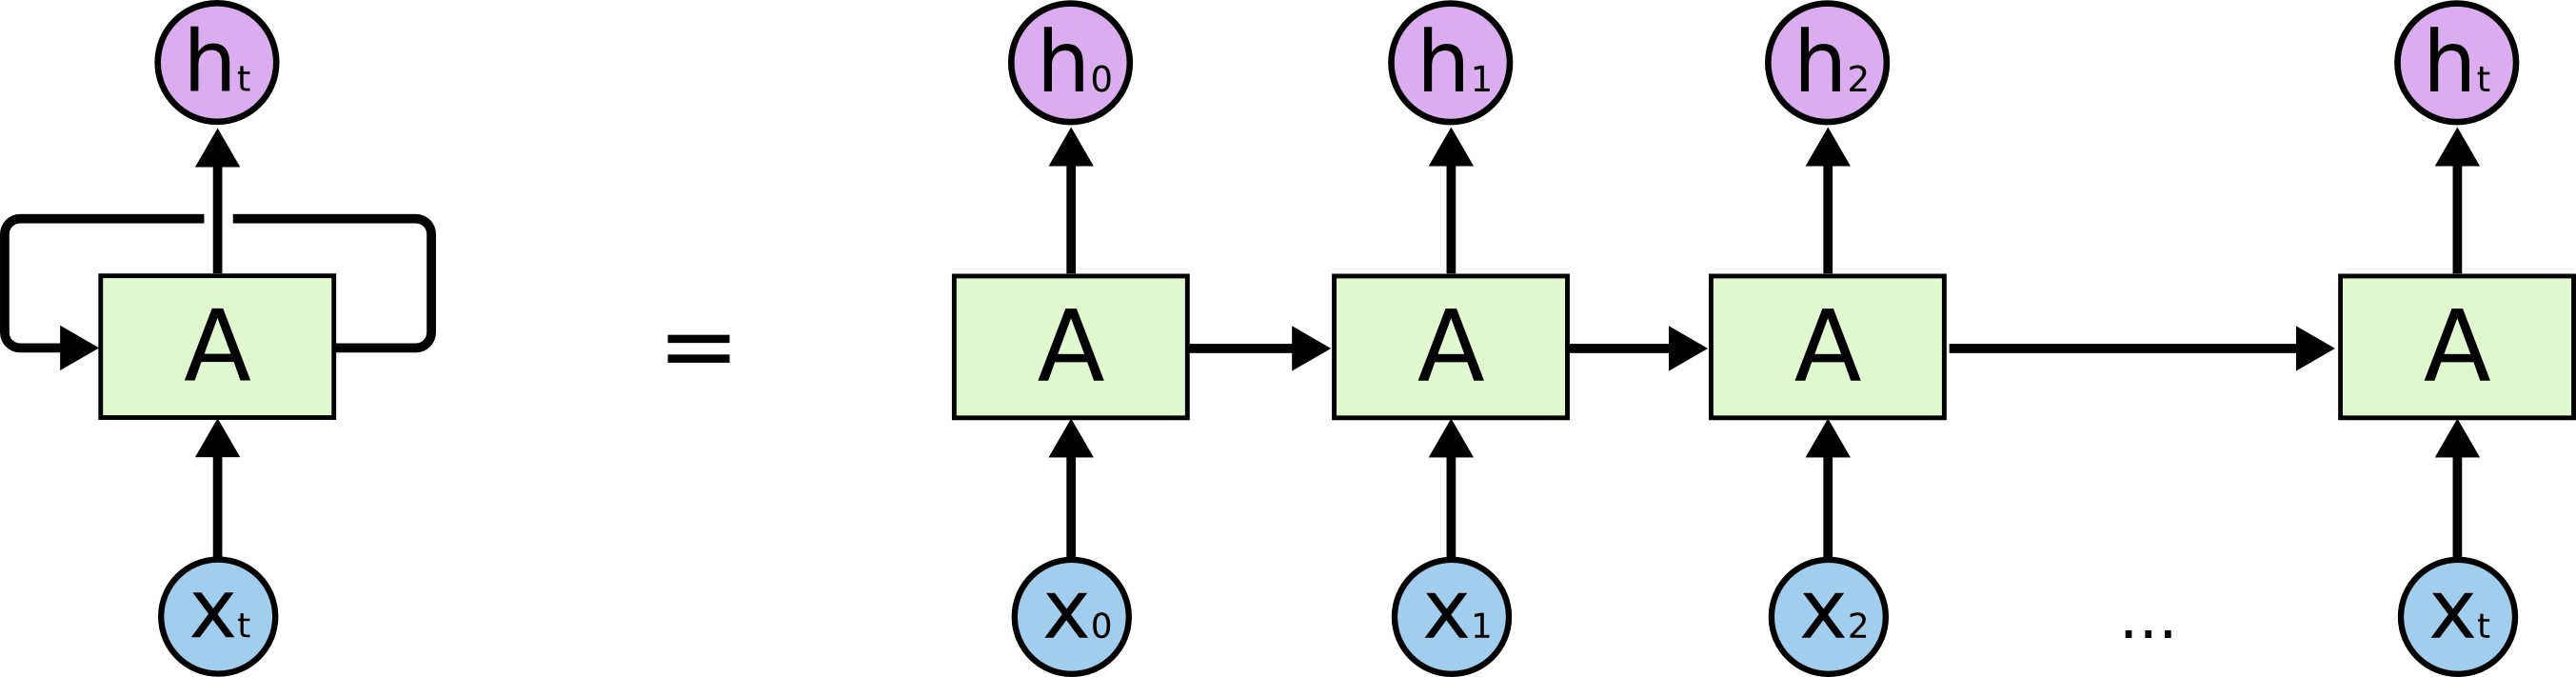
\includegraphics[width=0.95\textwidth]{rnnUnrolled.png}}
\caption[Unrolled RNN]{
    An RNN unrolled into a neural network with t+1 layers \cite{rnnUnrolled}
}
\label{fig:rnnUnrolled}
\end{figure}


Some applications for which RNNs have proven useful include speech transcription, machine translation (translating one language to another), video frame classification, and image captioning \cite{rnn}.  These applications all require the RNNs' stateful transitioning while processing the sequence of input; for example, producing a valid translation greatly depends on the part of sentence previously translated.  Furthermore, RNNs have also proven themselves to be highly performant in the absence of sequential input, as was the case in DeepMind's RNN that transcribed house numbers from Google Street View \cite{deepMindHouseNumber}.


\begin{figure}[h]
\centering
\captionsetup{justification=centering,width=0.95\textwidth}
\centerline{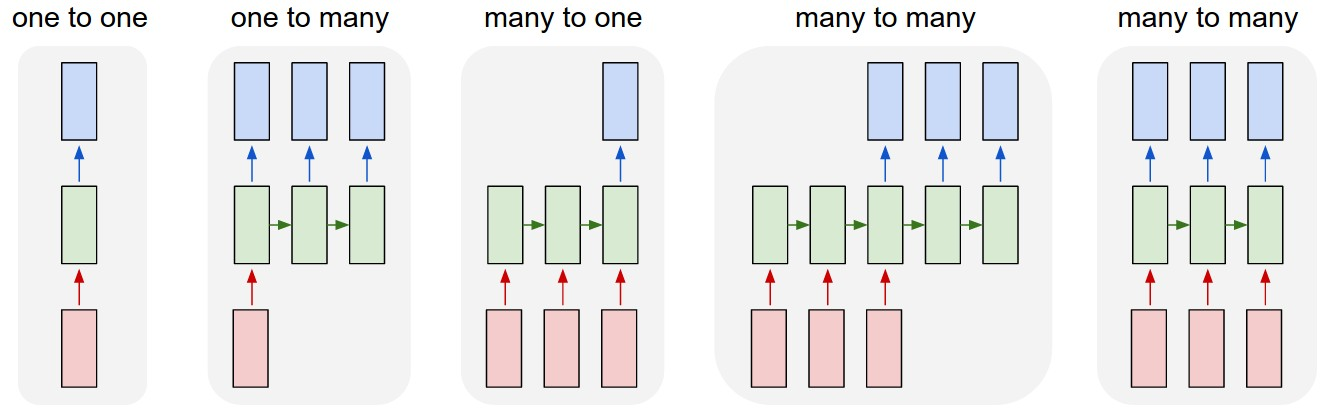
\includegraphics[width=0.95\textwidth]{rnnTransformations.png}}
\caption[Various RNN Setups]{
    The various use-cases for RNNs (green blocks) using input vectors (red) to produce output (blue) \cite{rnnTransformations}
}
\label{fig:rnnTransformations}
\end{figure}


As shown by Fig. \ref{fig:rnnTransformations}, RNNs can be used in a variety of settings.  The left-most setup ("one to one") demonstrates the transformation that occurs in typical neural networks: the input vector is processed completely by all of the hidden layers and then mapped to an output vector.  The "one to many" setup shows a transformation that may occur in settings like image captioning where a fix-sized image is transformed into a sequence of words.  The next setup, "many to one", illustrates how a sequential input is processed to produce a single label, which could be applied towards applications like sentiment classification.  The first "many to many" setup exemplifies the transformation that sentences could undergo in machine translation applications: input sequences are mapped to the target language using local context as opposed directly mapping each word independently.  Lastly, the second "many to many" configuration depicts a scenario in which an output is required for each constituent of the input sequence, e.g., a video classification task that requires labelling each frame \cite{rnnTransformations}.

However, there is a flaw with conventional RNNs.  The current state of an RNN, though dependent on previous parts of the input sequence, may be too far removed from the state at which a relevant piece of information was introduced.  For example, in the input sentence "I grew up in France... I speak fluent [language]", the RNN may not be able to predict "French" as the language since the word "France" occurred a lot earlier than where that information was actually necessary.  This gap between the necessary information and the point at which that information is actually needed may ultimately become too large for the RNN to be effective \cite{lstm}.  However, there is a special variant of the RNN, the long short-term memory (LSTM) network, that can overcome this limitation.

LSTMs are RNNs with special memory units (also known as cells) that can selectively keep information for an extended period of time \cite{lstmClassification}.  Instead of only consisting of a single repeating layer, as is the case with an RNN, the vanilla LSTM has one memory unit composed of four special layers: three sigmoid layers, and one tanh layer \cite{lstm}.  All sigmoid layers output values between 0 and 1, and the tanh layer outputs values between -1 and 1.  Together, these layers help the cell forget, remember, update, and produce information.

\begin{figure}[h]
\centering
\captionsetup{justification=centering,width=0.95\textwidth}
\centerline{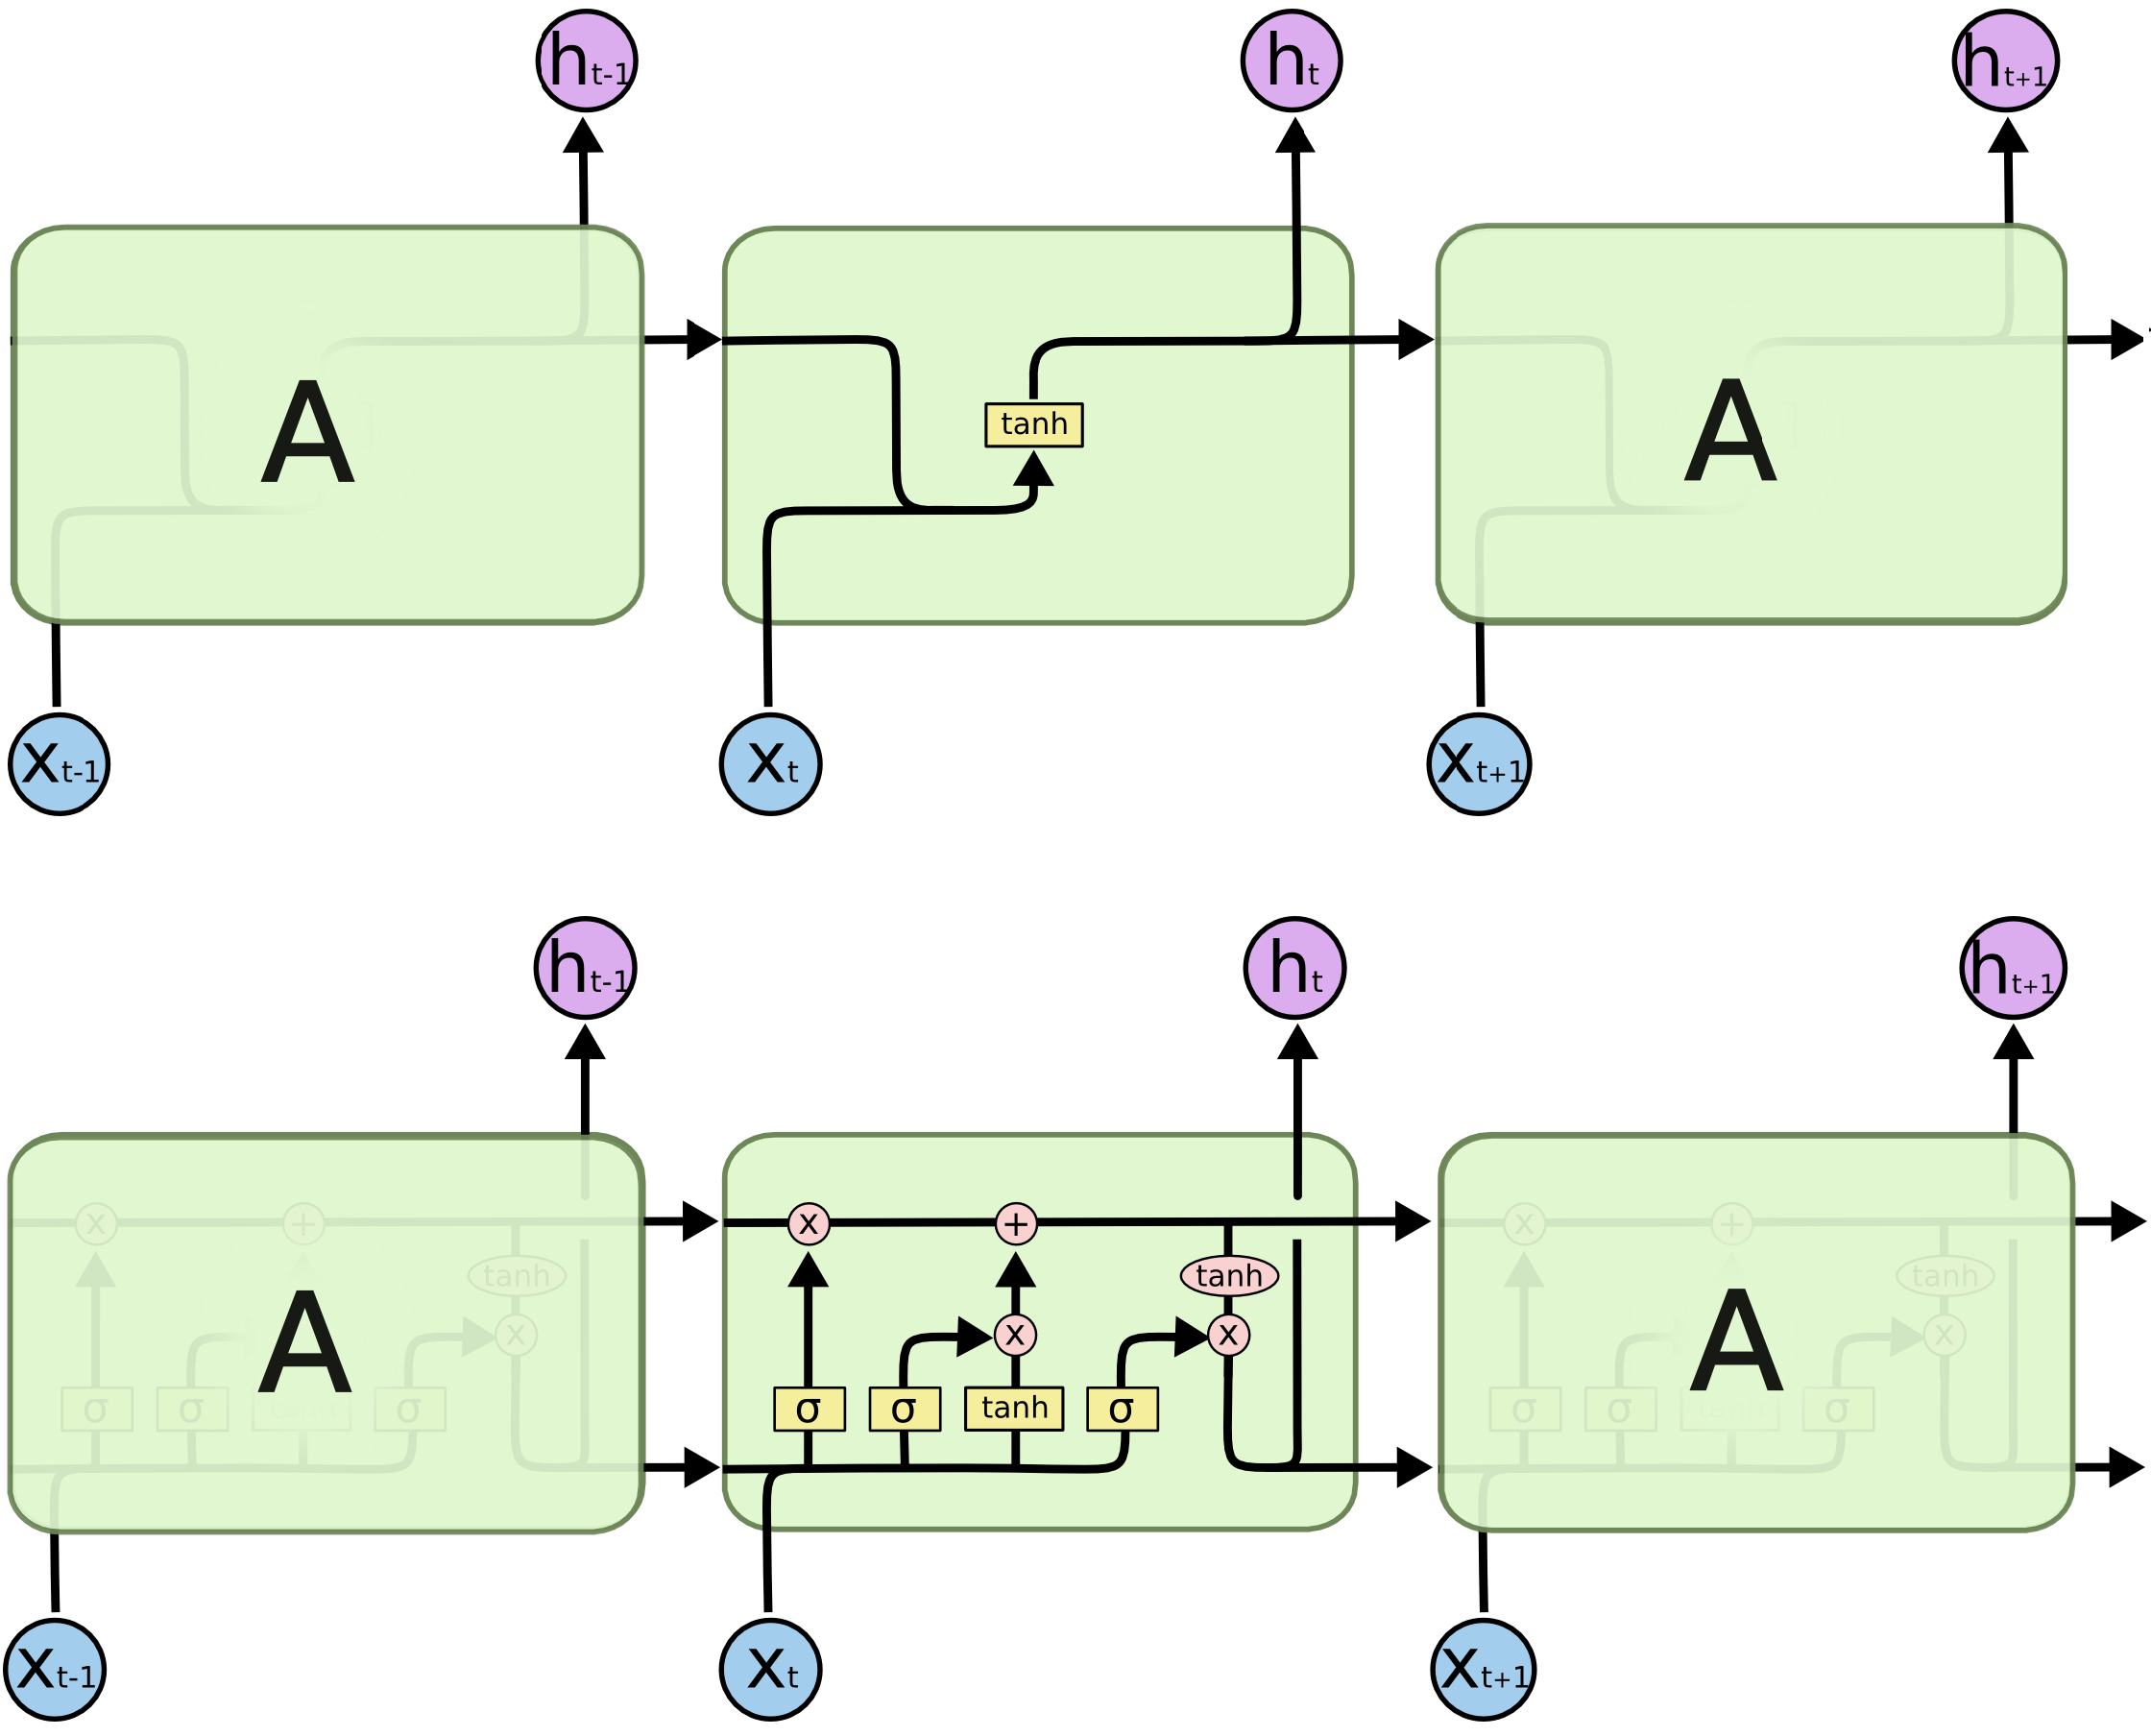
\includegraphics[width=0.95\textwidth]{rnnChainlstmChain.png}}
\caption[RNN Layer vs LSTM Layer]{
    Unrolled RNN and LSTM chains\\
    Top: RNN with a single layer in each state \cite{rnnChain}\\
    Bottom: LSTM with one memory unit in each state \cite{lstmChain}
}
\label{fig:lstmChain}
\end{figure}

As shown in the LSTM in Fig. \ref{fig:lstmChain}, the first layer is a sigmoid layer whose input is the concatenation of the output from the previous state (\textbf{h\textsubscript{t-1}}) and the current input (\textbf{x\textsubscript{t}}).  In LSTMs, sigmoid layers that are joined with pointwise multiplication operators act as gates that let information through whenever their outputs are non-zero values.  The first sigmoid layer uses \textbf{h\textsubscript{t-1}} and \textbf{x\textsubscript{t}} and forms a gate on the incoming stream of values from the previous cell state (the top left corner of each cell in Fig. \ref{fig:lstmChain}).  This gate, often called the "forget gate", outputs a number between 0 and 1 for each value in the previous state.  Thus, if the gate outputs 0 for a particular value, that value is completely forgotten.

The next stage of the cell decides how much of the new information (\textbf{h\textsubscript{t-1}} and \textbf{x\textsubscript{t}}) will be retained in the state.  First, a tanh layer is used to compute an updated value for each bit of new information.  Afterwards, these updated values are filtered by another gate in order to extract whatever is deemed pertinent by the LSTM.  Finally, the filtered information is added with whatever information from the previous state that was not forgotten to form the new cell state.

The last stage of the cell computes the output for the current state (\textbf{h\textsubscript{t}}).  The first step in this stage is to map the cell state into the acceptable output space.  In Fig. \ref{fig:lstmChain}, the tanh activation function is applied to the cell state to push each value between -1 and 1.  The transformed state is then passed through the final sigmoid gate; thus, the output consists of only the parts of the cell state the LSTM deems appropriate.  For example, in a machine translation setting, the LSTM may output whether or not the subject is singular or plural, so the LSTM knows how to conjugate the following verb if that is in fact the following input \cite{lstm}.

There are other LSTM configurations, and each has its own advantages in certain settings.  However, a recent study shows that most of these variations do not perform significantly better than the vanilla LSTM \cite{variousLSTMs}.  The LSTM model used in this thesis is a variant of the vanilla LSTM model that has a configurable number of memory units \cite{kerasLSTM}.  Note that the LSTM presented in this section only had a single memory unit, and, thus, produced a single output.  Adding extra memory units increases the dimensionality of the output at each state.  Thus, if the LSTM contains 50 memory units in each layer, the LSTM will ultimately produce a 50-dimensional output vector after processing the entire input sequence.  Since the challenge presented in this thesis is a binary classification task, the outputs of each LSTM are passed through another sigmoid activation layer to produce a prediction.


\chapter{Related Work}

The current approaches to validating news and facts and filtering out unreliable content are currently limited, but there is a good foundation for future systems to build on.  These approaches either attempt to verify content independently, or use prior knowledge and biases to block out suspicious sources completely, usually after user complaints.  For example, organizations like Snopes and PolitiFact employ professionals to verify claims manually, and universities usually post guidelines for their students on how to recognize trustworthy sources of information.  Even Facebook turned to third-party fact-checking organizations, including Snopes and PolitiFact, to flag disputed stories in an attempt to stem the tide of a viral fake news story \cite{fighingFakeNews}.  However, given the speed at which sensational news travels, waiting on journalists to perform thorough research is not entirely feasible and the reader must do their own due diligence.


\section{Manual Fact Checking and Source Validation}

Snopes and PolitiFact are two prominent and well-respected fact checking organizations that regularly post fact checks on controversial issues.  Snopes.com is a completely independent and self-sufficient website that was launched in 1994 by David Mikkelson to host his research on the prevalent urban legends of his time.  Since then, Snopes has since grown into a resource that many people, including journalists, rely on for credible information \cite{snopesAbout}.  PolitiFact is much more recent product and focuses primarily on fact-checking elected officials and others in the public eye who speak about politics.  PolitiFact is run by editors and reporters from the \textit{Tampa Bay Times}, an independent newspaper, and is owned by the non-for-profit Poynter Institute, a school for journalism in Florida \cite{politifactAbout}.  Though both organizations share a similar mission of informing their readers, PolitiFact chooses to only analyze the most newsworthy political claims while Snopes chooses whichever topics their readers are most interested in at any given time.

For a more immediate sense on the veracity of an article, readers can either dig into the claims made in the article themselves, or use basic guidelines to be decide how wary or suspicious they should be of the publishing source.  One relevant resource cited by Harvard Library's Research Guides is OpenSources.co, an ongoing project that retains an updated registry of misleading and fake news \cite{harvardResearch}.  Led by Dr. Melissa Zimdars at Merrimack College, the OpenSources team analyzes each source to determine the lack of transparency, level of inaccuracy, extreme bias, and other indications of purposeful misinformation.  Some of the labels they use to tag untrustworthy sources are "fake" for sources that fabricate stories, "bias" for sources that have an extreme political view and often decontextualize information, "hate" for sources that actively promote racism, misogyny, homophobia and other forms of discrimination.  The labels they use to tag potentially trustworthy sources are "political" for sources that provide verifiable information for certain political views, and "reliable" for sources that post information "in a manner consistent with traditional and ethical practices in journalism" \cite{opensources}.

OpenSources' steps for labelling include analysis of the title and domain, publishing author and sources cited (if any), writing style, aesthetics of the web page, and the source's social media presence.  For example, if the title or domain seems like an imitation of a more prominent news authority, or the web page seems like a misshapen blog, it is highly likely that the website is not a credible source of reliable information.  Furthermore, if the writing style seems inconsistent, is grammatically incorrect, or contains a lot of capital words with exclamation marks, the article may be clickbait and purposefully incendiary to invoke extreme feelings in the reader \cite{opensources}.

For an automated system to emulate the manual process that OpenSources contributors use for source tagging, the system would need to detect all the red flags a human would look out for.  However, since some of these markers are not easily quantifiable, this logic is not very formulaic and hinges on the discretion of the arbitrator, whether human or machine.  To overcome possible ambiguities, some systems, like browser extensions, just blacklist whole domains.  Other systems, like the one introduced in the following section, iteratively learns whether or not a source should be trusted.


\section{Knowledge Fusion}

In 2014, a research team at Google attempted to build a system capable of discerning truth from an aggregate of information scraped off of the web \cite{knowledgeFusion}.  They structured their study to tackle their newfound problem of identifying the probability that a scraped subject-predicate-object triple of information is actually true.  This challenge, which they called the knowledge fusion problem, builds on the data fusion problem which is the challenge of identifying the true values of data given a pool of conflicting information (e.g., determining President Obama's birthplace from a set of possible places extracted from different in articles, blogs, and editorials).  The motivation for the knowledge fusion problem is to use these true-labelled triples to build a web-scale knowledge base for fast and reliable information retrieval, similar to the knowledge graph used by the Google search engine.

Classical approaches to the data fusion problem predominantly determined truth values in accordance with either a voting scheme, rule-based system, a trustworthiness metric for quality-based labelling, or a source relationship-based method \cite{trustworthiness}.  The early rule-based systems updated truth values by mirroring the most recent source's value, or taking minimums, maximums, or averages for numerical values.  Quality-based approaches either rely on external metrics like page ranks and similarity scores, or compute likelihoods of correctness for the data.  The relation-based approaches try to establish links between sources by either attributing derivative sources with lower weights, or clustering sources into subsets to act as supporting evidence for particular data values.

The authors of "From Data Fusion to Knowledge Fusion" \cite{knowledgeFusion} experimented with adaptations to three data fusion techniques.  The first technique was a simple vote-based algorithm called VOTE that served as their baseline.  The other two techniques were statistical algorithms that learned sources' trustworthiness using the source's historical accuracy rate.  The trustworthiness of each source was then used to model the data values as a posterior distribution conditioned on the distribution of the data.  In each posterior distribution, the trustworthiness of the source serves as the likelihood of the value, and the distribution of the values serves as the prior probability \cite{popaccu}.

In the first statistical technique, called ACCU, a simplifying assumption is made that greatly reduces the complexity of the determining the prior probability; specifically, there are a constant number of uniformly distributed false values.  In contrast, the second technique, called POPACCU, derives the prior probability distribution of values using the observed data.  The authors chose POPACCU because it is more robust than ACCU in scenarios where sources copy each other \cite{popaccu}.  With enough false copycat sources, the distribution of false values becomes quite skewed and far from uniform.  To tackle the knowledge fusion problem, these data fusion techniques are modified to produce truthfulness probabilities as opposed to binary output: the ACCU techniques are modified to output their posterior probability, and the voting-based approach is modified to output the proportion of sources that agreed with the most popular value.

To evaluate their techniques, they use verified triples on Freebase, an open database of world knowledge \cite{freebase}, as their gold standard.  Triples of subject-predicate-object form (s-p-o) contained in Freebase are considered as always true, and s-p-o triples that are not in Freebase as a complete triple, but are seen as s-p pairs, are labelled false under the local closed-world assumption (LCWA).  In a closed-world system, all information is known by the system; however, in a LCWA system, the system only has complete knowledge about any local knowledge it contains.  Thus, if Freebase has knowledge of a particular data item (the s-p pair), under the LCWA assumption it has complete knowledge about that topic and so any triple formed using that subject-predicate is untrue if the triple is not already contained in Freebase.  Triples made of subject-predicate pairs that are not present in Freebase are ambiguous are simply excluded from the experiment \cite{knowledgeFusion}.

To numerically evaluate the performance of each technique, a precision versus recall plot is constructed.  The precision and recall are recorded as each new triple is extracted from a data source, and the area under this precision versus recall curve (AUC-PR) is used to describe the performance of each technique.  The results of their study show that the ACCU models have a better AUC-PR than VOTE.  The results also show that the VOTE technique usually underestimates the probability of true values.  That is, in scenarios where there are very few sources of data values, or none of the sources agree on any particular value, the confidence, or prediction probability, of the predicted value is quite low for VOTE.  This result stems from the fact that the VOTE technique does not learn to designate sources as trustworthy, and so when there are very few corroborating triples, VOTE has a low prediction confidence.  It turns out that ACCU has the highest AUC-PR, but slightly higher deviation between real probability and prediction probability as triples are iteratively added into consideration.

The results of this paper show that it is possible to make a fact-assessing system with high precision-recall if the system has immediate access to enough data from trustworthy sources.  However, this luxury is not available to any system that would wish to moderate news articles in realtime.  While the system in this study is far better solution than blacklisting whole domains, it may still develop a bias and excessively filter out articles.  For example, the system may be unfair to newer authors at organizations that have developed untrustworthy priors due to a few select publications.  This system may even unfairly block content from newer, unrecognized sources when they report breaking news that has not yet been corroborated.

Today, readers have almost a limitless number of sources for information - building a system that remembers the trustworthiness of each source, or tries to determine the source's trustworthiness based information previously published, if any, is infeasible.  A more feasible approach does not try to determine whether or not data is true, but instead tries to determine if the data is probably untrue based on how it is presented.



\chapter[Experimental Setup and Evaluation]{Experimental Setup \newline and Evaluation}

\section{Dataset Construction} \label{datasetConstruction}

In order to test the effectiveness of the machine learning algorithms and natural language processing techniques discussed in Chapter 2, we constructed a corpus of malicious and credible articles.  The malicious articles used in our dataset were all stories that had trended on social media that Snopes eventually investigated and labelled false.  A list of URLs to these articles was later compiled by Allcott and Gentzkow for their study on the impact of fake news on the 2016 presidential election \cite{gentzkow}.  After Dr. Gentzkow and his research assistant, Chuan Yu, provided us with this list, we designed a script to scrape the content of the article on each web page.  Of the 948 fake news URLs, just 478 articles that had gone live between January and December 2016 were still available at the start of this study (March 2017).

To compile a list of URLs to credible articles, we used the Google News search engine to query for news articles published by major news organizations.  In order to ensure that all the credible articles would be similar to the set of articles available during the campaign season, a few filters were applied to each query.  First, the keywords "trump", "clinton", and "election" were conjoined together with OR operators in each query to only capture articles related to the 2016 presidential election.  Next, a date range restriction from January 1, 2016 to December 1, 2016 was imposed on the query in ensure that the timespan of the credible corpus would be similar to that of the malicious corpus.  Finally, a Google News source filter was applied to the query to restrict the result set to articles that had actually been published by each of the following major news outlets: ABC, BBC, CBS, CNN, FOX, NY Times, Reuters, and Washington Post.

As shown in Fig. \ref{fig:googlenews}, the search results from Google News is not a list of URLs, but rather enriched content that includes thumbnails, articles' titles as hyperlinks, and short blurbs from each article.  Thus, a results page crawler was created to traverse through and extract the direct URLs from the first 17 pages of results returned by the aforementioned query for each news organization.  Once the crawler had curated a list of URLs to credible news articles, each corresponding web page was scraped for its news content.  At the end of this stage, 1226 credible articles had been successfully downloaded.


\begin{figure}[h]
\centering
\captionsetup{justification=centering,width=0.95\textwidth}
\centerline{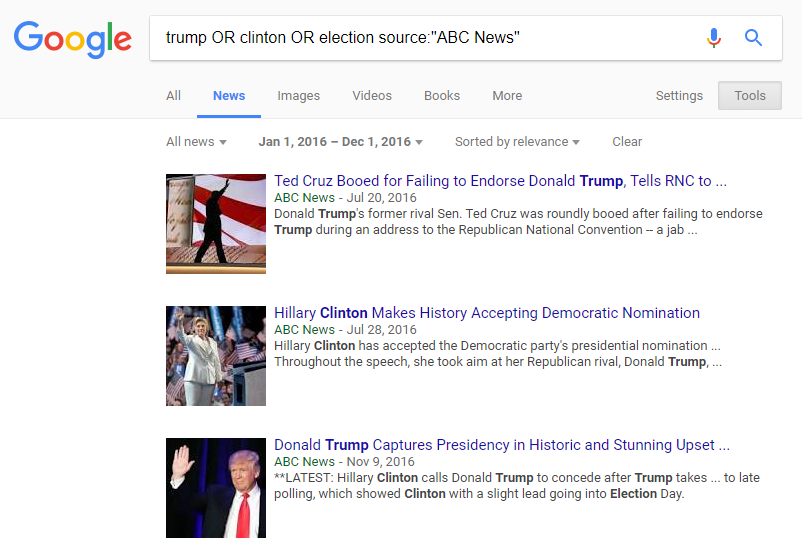
\includegraphics[width=0.95\textwidth]{googlenews.png}}
\caption[ABC News Articles On Google News]{
    Google News query results for articles published by ABC News between January 1, 2016 and December 1, 2016
}
\label{fig:googlenews}
\end{figure}


Hoping to reap the benefits of sentiment analysis that were discussed in Section \ref{sentimentAnalysisSection}, sentiment-related features for each document were added to the dataset using Google Cloud's Natural Language API and Microsoft Azure's Text Analytics API.  Though both APIs provide a sentiment score for each input document, their scores span across different ranges: Google's score lies between -1 and 1, and Microsoft's score lies between 0 and 1.  However, both APIs do indicate negative texts with low scores, and positive texts with high scores \cite{googleSentiment,microsoftSentiment}.  From here on out, an article is deemed negative if its Google sentiment score is less than -0.25 or if its Microsoft sentiment score is less than 0.375.  An article is considered positive if its Google sentiment score is greater than 0.25, or if its Microsoft sentiment score is greater than 0.625.  Additionally, we define polar articles as articles that are either negative or positive according to either API's sentiment score.

The other feature that the Google Cloud Natural Language API provides is the overall sentiment magnitude for the input text.  This magnitude, which ranges from 0 to infinity, indicates the overall strength of emotion in the text.  That is, each emotional word, whether it's positive or negative, additively contributes to the magnitude.  One drawback to this feature is that it is not normalized; thus, a document with a mix of sentiment and sentiment score close to 0 could potentially have a sentiment magnitude that is greater than the sentiment magnitude of a polar article simply because the mixed document is larger \cite{googleSentiment}.

To refine the overall dataset, duplicate documents and documents very similar to another document with the same label were eliminated.  To determine which documents are similar to others, a cosine similarity matrix of similarity scores (using tf-idf vector representation) between each pair of documents was constructed.  For each pair of documents with a similarity score greater than 0.90, the document that consisted of the least words was excluded from the dataset under the assumption that it was an article that simply quoting large chunks of the other with very little analysis.

After pruning the duplicate articles, a total of 333 malicious and 1008 credible articles remained.  In order create valid training and testing sets that reflected a possible real-world scenario, the dataset was ordered and split by date of publication.  That is, every article that was published before October 13, 2016 was moved into the training set, and every article that was published from October 13, 2016 and onwards was placed in the testing set.  Therefore, the training set is composed of the 774 of the earliest credible articles and 207 of the earliest malicious articles, and the testing set is composed of 234 of the newest credible articles and 126 of the newest malicious articles.  However, to further combat overfitting, a tuning set was ultimately broken off from the later 20\% of the training set; i.e., 154 of the latest credible articles and 41 of the latest malicious articles were removed from the training set and placed into the tuning set (a.k.a. validation set).  Thus, the actual training set consists of 620 oldest credible articles, and the 166 oldest malicious articles.


\section{Data Exploration} \label{dataExploration}

To determine which features may be the most effective for classification, the following plots are constructed to visualize the relationship between select features of the malicious and credible articles.


\begin{figure}[h!]
\centering
\captionsetup{justification=centering,width=0.95\textwidth}
\centerline{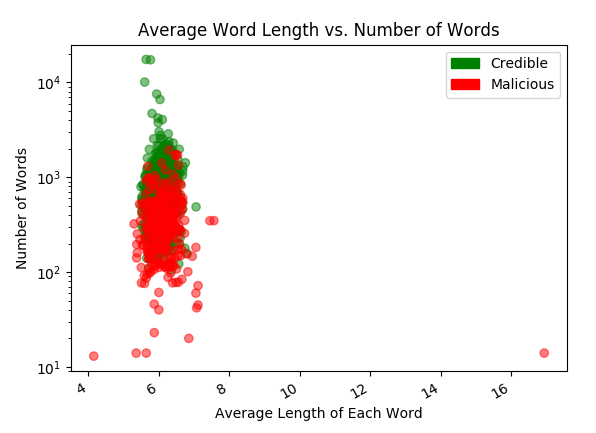
\includegraphics[scale=0.65]{wordlenNumWordsLogScale.png}}
\caption[Average Word Length vs Number of Words]{
    A plot of the average word length of each document and number of words in each document
}
\label{fig:wordlenNumWordsLogScale}
\end{figure}


\begin{figure}[h!]
\centering
\captionsetup{justification=centering,width=0.95\textwidth}
\centerline{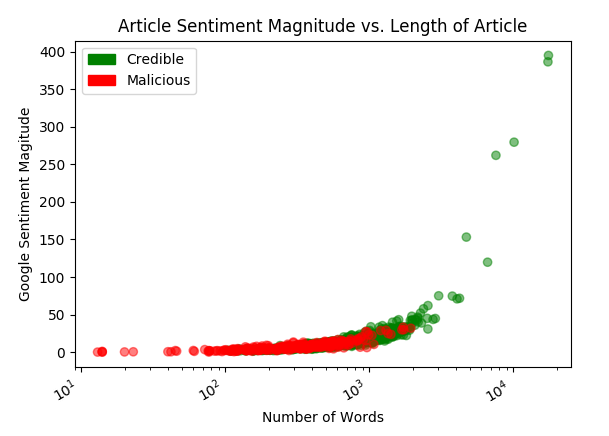
\includegraphics[scale=0.65]{sentimentMagnitude_vs_ArticleLen.png}}
\caption[Number of Words vs Google Sentiment Magnitude]{
    A plot of the number of words in each document and the Google sentiment magnitude of each document
}
\label{fig:numWordsToSentimentMagnitude}
\end{figure}


Fig. \ref{fig:wordlenNumWordsLogScale} shows the relationship between the average length of each word (i.e., the number of characters) in an article, and the number of words in the article.  Note that Fig. \ref{fig:wordlenNumWordsLogScale} has an outlier, all the way to right, representing a document with very long words, but with a few number of words.  This document that has an average word length greater than 16 characters exemplifies the wide range of styles for maliciously written web pages that pose as articles.  In fact, this particular document exhibits very few words, and simply points the reader to other links and tweets.

Fig. \ref{fig:numWordsToSentimentMagnitude} exemplifies the effect that the length of the document has on the Google sentiment magnitude.  As hypothesized before, larger documents tend to have a greater sentiment magnitude.  In fact, almost all of the credible articles that are longer than the longest malicious article has a sentiment magnitude greater than the sentiment magnitude of every malicious article.


\begin{figure}
\centering
\captionsetup{justification=centering,width=0.95\textwidth}
    \begin{subfigure}[h]{0.5\textwidth}
            \centering
            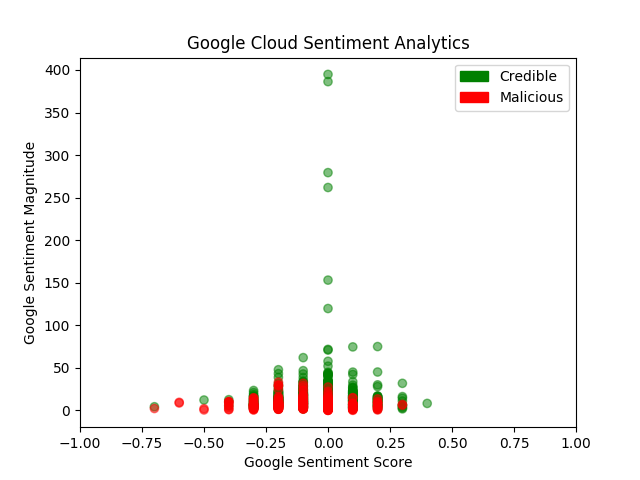
\includegraphics[width=\linewidth]{googleCloudSentiment.png}
            \caption[Google Sentiment Score vs Magnitude]{
                 Google Cloud Natural Language API 
            }
            \label{fig:googleCloudSentiment}
    \end{subfigure}\hfill
    \begin{subfigure}[h]{0.5\textwidth}
            \centering
            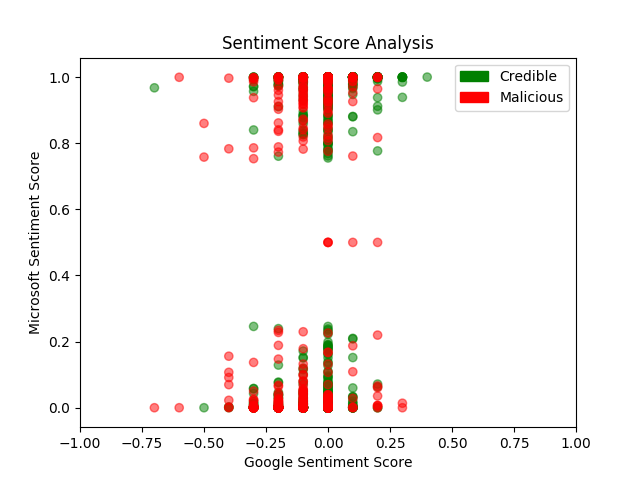
\includegraphics[width=\linewidth]{sentimentScoreAnalysis.png}
            \caption[Sentiment Scores: Google vs Microsoft]{
                Both APIs' sentiment scores
            }
            \label{fig:googleMicrosoftSentiment}
    \end{subfigure}\hfill
    \caption[Sentiment Analysis API Results]{
        Sentiment analysis results using Google Cloud and Microsoft Azure APIs
    }
\label{fig:sentimentScoreAnalysis}
\end{figure}


Fig. \ref{fig:googleCloudSentiment} depicts the shared relationship between the articles' Google sentiment score and magnitude, and Fig. \ref{fig:googleMicrosoftSentiment} shows the discrepancies between the sentiment scores according to different Google and Microsoft APIs.  If both sentiment analysis APIs were in complete agreement, the scatter plot would be roughly linear; i.e., articles attributed with a low Google sentiment score (approximately -1) should also have a correspondingly low correspond Microsoft sentiment score (approximately 0).  Even though the values seem contradictory at times, these features are kept in the dataset and the classifiers are charged with the task of learning appropriate weights for each feature in order to produce accurate predictions.


\begin{figure}
\centering
\captionsetup{justification=centering,width=0.95\textwidth}
    \begin{subfigure}[h]{0.5\textwidth}
            \centering
            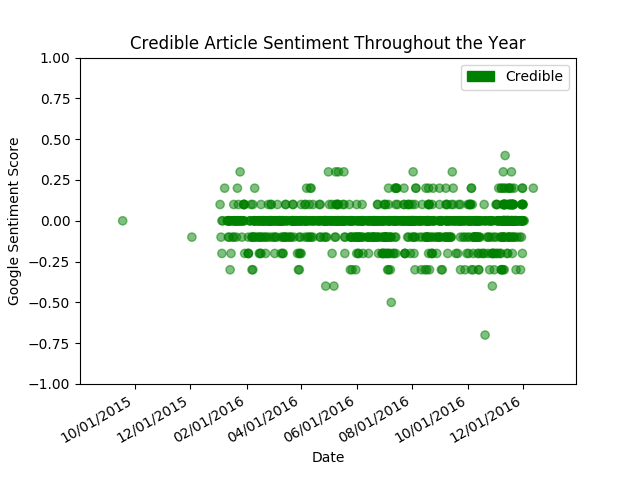
\includegraphics[width=\linewidth]{credibleSentimentThruYear.png}
            \caption{Credible Article Sentiment}
            \label{fig:credibleSentimentThruYear}
    \end{subfigure}\hfill
    \begin{subfigure}[h]{0.5\textwidth}
            \centering
            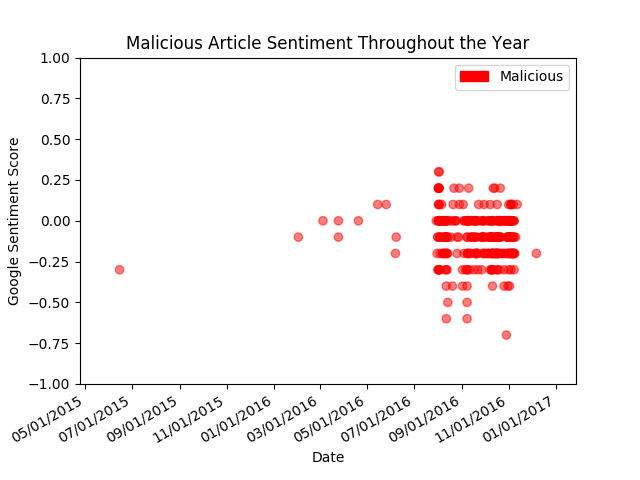
\includegraphics[width=\linewidth]{maliciousSentimentThruYear.png}
            \caption{Malicious Article Sentiment}
            \label{fig:maliciousSentimentThruYear}
    \end{subfigure}\hfill
    \caption[Article Sentiment Through Time]{
        Articles' sentiment from late 2015 to late 2016
    }
\label{fig:sentimentThruYear}
\end{figure}


Lastly, Fig. \ref{fig:sentimentThruYear} shows that distribution of Google Cloud sentiment scores throughout the date range encapsulated by the dataset.  Though most of the articles in both classes have Google sentiment scores that are relatively neutral, the proportion of malicious articles that are polar is substantially greater than the proportion of credible articles that are polar.  Only 48 of the 1008 credible articles (about 5\%) have a polar sentiment score.  On the other hand, 44 of the 333 malicious articles, or approximately 13\%, have an overall polar sentiment score.  This is a surprising statistic since credible articles also tend to have much higher sentiment magnitude.  One reason for this may be that traditional journalists try to avoid using hyperboles and stirring emotional responses \cite{opensources}.  Since the journalists who authored the credible articles tend to balance their usage of polarizing words, their articles should be more neutral than articles written by unscrupulous authors, like the Russian nationals who sought to undermine the campaigns \cite{russianBots}.

\section{Evaluation Metrics} \label{evaluationMetricsSection}

There are a variety of metrics for quantifying the performance of machine learning classifiers.  Some well-known metrics used to evaluate a classifier are overall accuracy,  precision, recall, and F1-score.  The overall accuracy (Eq. \ref{eq:overallAccuracy}), which is simply the proportion of correct classifications, is not an ideal evaluation metric for applications with large class imbalances since high accuracy scores can easily be obtained by just labelling all test documents as the class with the greatest population density.  Since the proportion of credible articles is much greater than the proportion of malicious articles, a classifier with a moderately high accuracy can still turn out to be a poor detector of malicious articles.  Thus, this study will highlight each classifier's class and prevalence-weighted average precision, recall, and F1-score due to their relationship between the number of true positives ($t_{p}$), false positives ($f_{p}$), and false negatives ($f_{n}$) produced by the classifier\cite{pythonMetrics}.

\begin{equation}
\label{eq:overallAccuracy}
\mbox{overall accuracy} = \frac{t_{p}(\mbox{credible}) + t_{p}(\mbox{malicious})}{N}, N = \mbox{size of test set}
\end{equation}
\begin{equation}
\label{eq:classPrecision}
\mbox{precision}_{c} = \frac{t_{p, c}}{t_{p, c} + f_{p, c}}
\end{equation}
\begin{equation}
\label{eq:classRecall}
\mbox{recall}_{c} = \frac{t_{p, c}}{t_{p, c} + f_{n, c}}
\end{equation}
\begin{equation}
\label{eq:classF1Score}
\mbox{F1-score}_{c} = 2 \cdot \frac{\mbox{precision}_{c} \cdot \mbox{recall}_{c}}{\mbox{precision}_{c} + \mbox{recall}_{c}}
\end{equation}
\begin{equation}
\label{eq:classProportion}
p_{c} = \frac{|D_{c}|}{N} = \frac{\mbox{number of test articles of class}\ c}{\mbox{number of test articles}}
\end{equation}
\begin{equation}
\label{eq:avgPrecision}
\mbox{weighted avg. precision} = (\mbox{precision}_{c_{0}}*p_{c_{0}}) + (\mbox{precision}_{c_{1}}*p_{c_{1}})
\end{equation}
\begin{equation}
\label{eq:avgRecall}
\mbox{weighted avg. recall} = (\mbox{recall}_{c_{0}}*p_{c_{0}}) + (\mbox{recall}_{c_{1}}*p_{c_{1}})
\end{equation}
\begin{equation}
\label{eq:avgF1Score}
\mbox{weighted  avg. F1-score} = (\mbox{F1-score}_{c_{0}}*p_{c_{0}}) + (\mbox{F1-score}_{c_{1}}*p_{c_{1}})
\end{equation}


The class precision (Eq. \ref{eq:classPrecision}) is the ratio of the true positives to the total number of predicted positives and indicates how often the classifier's prediction of a class was accurate.  The class recall (Eq. \ref{eq:classRecall}), also known as the sensitivity, is the ratio of true positives to total number documents in the class.  The recall of a class is indicative of the classifier's ability to find all the documents of that class.  To combine both the precision and recall, the class F1-score (Eq. \ref{eq:classF1Score}) is computed as the harmonic mean of both.  Finally, the prevalence-weighted average of each of these scores (Eq. \ref{eq:avgPrecision} - \ref{eq:avgF1Score}) is computed using the sum of each class score weighted by its class proportion (Eq. \ref{eq:classProportion}).  Thus, the average F1-score will be used to decide which approach works best since the average score proportionally reflects the performance of the model on each class of articles.


\section{Model Construction and Evaluation} \label{modelConstruction}

Using the training, tuning, and testing sets described in Section \ref{datasetConstruction}, we trained and evaluated the KNN, SVM, and LSTM algorithms.  The following subsections discuss how each classifier was tuned to obtain the optimal performance, and state the results of each classifier.


\subsection{$K$-Nearest Neighbor} \label{KNNResults}

The central parameter of the KNN classifier, introduced in Section \ref{knnSection}, is $k$, the number of closest neighbors used to predict the class for each document in the test set.  To train the baseline KNN classifier, only the tf-idf weights of each document were used as input.  This baseline was then trained and tested with a variety of values for $k$, as well as Euclidean distance, Manhattan distance, and cosine distance as the comparison metric, to determine the optimal model.  This tf-idf model was constructed using each article's textual content after it was preprocessed to ensure that it was converted to lowercase and tokenizable by whitespace.  Surprisingly, the optimal baseline KNN model for this setting used only 1 neighbor ($k$ = 1) and the Euclidean distance metric.  This KNN model managed to achieve an overall accuracy of 0.75 and an average F1-score of 0.71 (refer to Table \ref{table:baselineKNN} for the complete classification report using the metrics discussed in Section \ref{evaluationMetricsSection}).  For the exact number of true positives, false positives, and false negatives for each class, refer to the confusion matrix in Table \ref{table:baselineKNNConfusion}.


\begin{table}[h!]
\centering
\begin{tabular}{|c | c  c  c | c|}
\hline
class      & precision & recall & F1-score & support\\
\hline
credible   & 0.73      & 1.00   & 0.84     & 234    \\
malicious  & 0.97      & 0.30   & 0.46     & 126    \\
\hline
average    & 0.81      & 0.75   & 0.71     &   \\
\hline
\end{tabular}
\caption[Baseline KNN's Classification Report]{Classification results of the baseline KNN model (trained using only the tf-idf weights as the input feature vector, $k$ = 1, and the Euclidean distance metric)}
\label{table:baselineKNN}
\end{table}


\begin{table}[h!]
\centering
\begin{tabular}{|c | c  c | c|}
\hline
                Actual class & 
                Predicted credible 
                &   
                Predicted malicious
                & support\\
\hline
credible   & 233                & 1                   & 234\\
malicious  & 88                 & 38                  & 126\\
\hline
total      & 321                & 39                  & 360\\
\hline
\end{tabular}
\caption[Baseline KNN's Confusion Matrix]{Confusion matrix for the baseline KNN model}
\label{table:baselineKNNConfusion}
\end{table}


The next KNN classifier was trained using feature vectors composed of the number of characters, number of words, Google sentiment score, Google sentiment magnitude, and Microsoft sentiment score of each training article.  The optimal model, which used $k$ = 5 and Manhattan distance, obtained an overall accuracy of 0.75 and an average F1-score of 0.72 (refer to Table \ref{table:secondKNN} for class-specific metrics).


\begin{table}[h]
\centering
\begin{tabular}{|c | c  c  c | c|}
\hline
class      & precision & recall & F1-score & support\\
\hline
credible   & 0.74      & 0.93   & 0.83     & 234    \\
malicious  & 0.76      & 0.40   & 0.53     & 126    \\
\hline
average    & 0.75      & 0.75   & 0.72     &   \\
\hline
\end{tabular}
\caption[Second KNN's Classification Report]{Classification results of the second KNN model (trained using all of the sentiment features, as well as the word and character counts, $k$ = 5, and the Manhattan distance metric)}
\label{table:secondKNN}
\end{table}


\begin{table}[h!]
\centering
\begin{tabular}{|c | c  c  c | c|}
\hline
class      & precision & recall & F1-score & support\\
\hline
credible   & 0.75      & 0.94   & 0.83     & 234    \\
malicious  & 0.79      & 0.42   & 0.55     & 126    \\
\hline
average    & 0.76      & 0.76   & 0.73     &   \\
\hline
\end{tabular}
\caption[Final KNN's Classification Report]{Classification results of the final KNN model (trained using tf-idf weights of each document, the number of characters and words in the document, the Google sentiment score and magnitude for the document, and the Microsoft sentiment score, $k$ = 7, and the Euclidean distance metric)}
\label{table:lastKNN}
\end{table}


Finally, another KNN classifier was trained using the tf-idf weights vector of each document, as well as all of the sentiment and count-related features used by the second KNN.  This classifier managed to achieve an overall accuracy of 0.76 and an average F1-score of 0.73 using $k$ = 7 and Euclidean distance (refer to Table \ref{table:lastKNN} for more metric scores).


\subsection{Support Vector Machine} \label{SVMResults}

Three SVMs were trained using the same setup that was used to train the three KNNs in Section \ref{KNNResults}.  The baseline SVM used only the tf-idf weights vector of each document as the input during training and testing, the next SVM used character and word counts along with the sentiment features of each document, and the final SVM used all of the features including the tf-idf weights.


\begin{table}[h]
\centering
\begin{tabular}{|c | c  c  c | c|}
\hline
class      & precision & recall & F1-score & support\\
\hline
credible   & 0.85      & 1.00   & 0.92     & 234    \\
malicious  & 1.00      & 0.67   & 0.81     & 126    \\
\hline
average    & 0.90      & 0.89   & 0.88     &   \\
\hline
\end{tabular}
\caption[Baseline SVM's Classification Report]{Classification results of the baseline SVM model (trained using only the tf-idf weights of each document, a linear kernel function, and $C$ = 1.0)}
\label{table:baselineSVM}
\end{table}


\begin{table}[h]
\centering
\begin{tabular}{|c | c  c | c|}
\hline
                Actual class & 
                Predicted credible 
                &   
                Predicted malicious
                & support\\
\hline
credible   & 234                & 0                   & 234\\
malicious  & 41                 & 85                  & 126\\
\hline
total      & 275                & 85                  & 360\\
\hline
\end{tabular}
\caption[Baseline SVM's Confusion Matrix]{Confusion matrix for the baseline SVM model}
\label{table:baselineSVMConfusion}
\end{table}


The optimal baseline SVM achieved an overall accuracy of 0.89 and an average F1-score of 0.88 using a linear kernel function, and regularization parameter ($C$) of 1.0 \cite{svcDoc}.  For a complete summary of the performance of the baseline SVM, refer to Table \ref{table:baselineSVM}.  Note that the performance of this baseline is much better than that of the baseline KNN (recall that the baseline KNN achieved an average F1-score of just 0.71).  The confusion matrix in Table \ref{table:baselineSVMConfusion} provides an explanation for this phenomenon: every credible article was correctly identified by the SVM, and more than twice as many malicious articles were successfully detected by the SVM than the KNN.

Unlike the improvement that the second KNN showed over the baseline KNN, the second SVM, trained without the tf-idf weights, performed significantly worse than the baseline SVM.  The overall accuracy of this new SVM model was 0.75, and its average F1-score was only 0.71.  This model used a radial basis kernel function, gamma of 0.0005 (the coefficient on the radial basis kernel), and $C$ = 1.0 (refer to Table \ref{table:secondSVM} for a complete summary of the SVM's performance).


\begin{table}[h!]
\centering
\begin{tabular}{|c | c  c  c | c|}
\hline
class      & precision & recall & F1-score & support\\
\hline
credible   & 0.73      & 0.96   & 0.83     & 234    \\
malicious  & 0.82      & 0.36   & 0.50     & 126    \\
\hline
average    & 0.76      & 0.75   & 0.71     &   \\
\hline
\end{tabular}
\caption[Second SVM's Classification Report]{Classification results of the second SVM model (trained using all of the sentiment features, as well as the word and character counts, a radial basis function, gamma = 0.0005, and $C$ = 1.0)}
\label{table:secondSVM}
\end{table}


The final SVM, which used each document's tf-idf weights in conjunction with the number of characters and words, and the Google and Microsoft sentiment features for the document, showed slight improvement over the second SVM.  This SVM, trained with a radial basis function, a gamma of 0.0001, and $C$ = 0.5, ultimately obtained an overall accuracy of 0.76 and an average F1-score of 0.73.  For the class precision, recall, and F1-scores, refer to Table \ref{table:lastSVM}.


\begin{table}[h]
\centering
\begin{tabular}{|c | c  c  c | c|}
\hline
class      & precision & recall & F1-score & support\\
\hline
credible   & 0.75      & 0.97   & 0.84     & 234    \\
malicious  & 0.86      & 0.39   & 0.54     & 126    \\
\hline
average    & 0.79      & 0.76   & 0.73     &   \\
\hline
\end{tabular}
\caption[Final SVM's Classification Report]{Classification results of the final SVM model (trained using tf-idf weights of each document, the number of characters and words in the document, the Google sentiment score and magnitude for the document, and the Microsoft sentiment score, a radial basis function, gamma = 0.0005, and $C$ = 1.0)}
\label{table:lastSVM}
\end{table}


\subsection{Long Short-Term Memory Network}

The last model evaluated in this study was the LSTM.  As discussed in Section \ref{rnnSection}, LSTMs have proven to be successful in tasks involving sequential information because of their memory units.  However, the input vectors used with the other classifiers, such as the tf-idf weights vector, do not retain any information about the sequential relationship between the words and sentences that make up each document.  Thus, the more reasonable input for LSTMs are sequences of word embedding vectors; in fact, word embeddings are the preferred choice for textual representation in modern deep learning \cite{wordEmbedding}.

Using the training and tuning set, we tuned LSTM's number of memory units, number of epochs, batch size, and input and recurrent dropout rates.   The number of epochs is the number of times the entire training set is passed forward and backward through the neural network.  If the number of epochs is too low, the network may be underfit and the resulting neuron weights will be far from optimal.  The batch size is simply the number of samples fed into the network before each update to the weights and helps to make training more efficient by reducing the memory requirements and the number of iterations required to reach the optimal weights \cite{batchSize}.  Finally, the dropout rate is simply probability that an input or recurrent node is excluded from consideration during a weight update in an effort to reduce overfitting \cite{dropoutRate}.


\begin{table}[h]
\centering
\begin{tabular}{|c | c  c  c | c|}
\hline
class      & precision & recall & F1-score & support\\
\hline
credible   & 0.90      & 0.95   & 0.93     & 234    \\
malicious  & 0.90      & 0.80   & 0.85     & 126    \\
\hline
average    & 0.90      & 0.90   & 0.90     &   \\
\hline
\end{tabular}
\caption[LSTM's Classification Report]{Classification results of the top-performing LSTM (overall accuracy of 0.90) using batch size of 24, 8 epochs, dropout rate of 0.5, and 50 memory units}
\label{table:lstmResults}
\end{table}

\begin{table}[h]
\centering
\begin{tabular}{|c | c  c | c|}
\hline
                Actual class & 
                Predicted credible 
                &   
                Predicted malicious
                & support\\
\hline
credible   & 223                & 11        & 234\\
malicious  & 25                 & 101       & 126\\
\hline
total      & 256                & 104       & 360\\
\hline
\end{tabular}
\caption[LSTM Confusion Matrix]{Confusion matrix for the LSTM model trained using 50 memory units, batch size of 24, a dropout rate of 0.5, and 8 epochs}
\label{table:lstmConfusion}
\end{table}

As illustrated by Table \ref{table:lstmResults}, the LSTM achieves an overall accuracy of 0.90, as well as an average F1-score of 0.90, with just 50 memory units, a batch size of 24, and 8 epochs.  According to the LSTM's confusion matrix (Table \ref{table:lstmConfusion}), the LSTM has 11 more false negatives for the credible class of articles than the SVM model, but 16 fewer false negatives for the malicious class of articles.


\chapter{Conclusion}

\section{Discussion of Results}

The top performing model is the LSTM that uses the word embedding representation of each article.  The LSTM's high average F1-score (0.90) indicates that the LSTM is adept at differentiating between credible and malicious articles.  The baseline SVM, which only used tf-idf weights of each document, also performed very well and obtained an overall F1-score of 0.88.  Interestingly, the addition of the sentiment analysis features adversely impacted the performance of the SVM, whereas the addition of these features improved the performance of the KNN system.

The success of the LSTM in this study exemplifies the LSTM's ability to encapsulate some of the nuances ingrained in text.  Since the LSTM was only given the word embedding representation of each article, it does not rely sentiment or any other non-textual features.  Instead, the LSTM churns through text in the sequential order it was written, much like a human reader, and gives its prediction after all the content has been consumed.


\section{Future Work}

This study examines the feasibility of using well known machine learning algorithms to tackle the growing threat of fake news, by distinguishing between accurate, trustworthy information and malicious content.  Since this study focused only on the articles that surfaced during the United States' 2016 presidential campaign, the impact of the findings presented here may only be applicable to a small subset of misinformation that poses as fact online.  Further analysis needs to be done to see if the approaches presented in this study can be applied or modified to a broader range of domains.  Ideally, the algorithms, particularly the LSTM, are general enough to work with minimum adjustments, like retuning and retraining with a larger dataset that adequately reflects the new population.

Another limitation of this study is its heavy reliance on articles tagged by Snopes.  Since the malicious corpus is comprised of articles identified as fake by only one source, the sampling methodology exhibits selection bias, even though Snopes itself is a credible arbitrator.  Therefore, future studies should incorporate articles with a greater consensus from accepted arbitrators, as well as expand their corpora with more recent news.

This study sought to show that it is possible to create an unbiased system capable of filtering out fake, or maliciously written, news by using only the articles' content, and not any preconceived notions about the source.  More work still needs to be done improve the performance of the techniques used in this study, as well as the number of domains that these techniques can be applied to.  Lastly, future studies that tackle the surge of fake news should be beyond reproach.  To successfully diminish the effects of fake news injected into social media by malicious content creators, the system must be fair, robust, and always learning.



% Bibliography
\clearpage

\addcontentsline{toc}{chapter}{Bibliography}

%\pagestyle{plain} % Remove all the special formatting in the fancyhdr

\fancyhead[LO]{\textit{Bibliography}}
\fancyhead[RO]{}

\begin{thebibliography}{99}
\raggedright


\bibitem{politifactAbout}
Adair, B., \& Holan, A. D. (2013, November 1). The Principles of PolitiFact, PunditFact and the Truth-O-Meter. Retrieved from \url{http://www.politifact.com/truth-o-meter/article/2013/nov/01/principles-politifact-punditfact-and-truth-o-meter/}

\bibitem{gentzkow}
Allcott, H., \& Gentzkow, M. (2017, January). Social Media and Fake News in the 2016 Election. Retrieved from \url{https://web.stanford.edu/~gentzkow/research/fakenews.pdf}

\bibitem{deepMindHouseNumber}
Ba, J., Minh, V., \& Kavukcuoglu, K. (2015, April 23). Multiple Object Recognition with Visual Attention. Retrieved from \url{https://arxiv.org/pdf/1412.7755.pdf}

\bibitem{rnnUnfolding}
Bengio, Y., Hinton, G., \& LeCun, Y. (2015, September 17). \textit{A Recurrent Neural Network and the Unfolding in Time of the Computation Involved in its Forward Computation} [Digital image]. Retrieved from \url{https://images.nature.com/full/nature-assets/nature/journal/v521/n7553/images/nature14539-f5.jpg}

\bibitem{rbfKernel}
Bernstein, M. (2017, March 28). The Radial Basis Function Kernel. Retrieved from \url{http://pages.cs.wisc.edu/~matthewb/pages/notes/pdf/svms/RBFKernel.pdf}

\bibitem{bishop}
Bishop, C. M. (2006). Kernel Methods, \textit{Pattern Recognition and Machine Learning} (p. 292). New York, NY: Springer.

\bibitem{englandFakeNews}
Booth, W. (2017, November 14). Britain's May Slams Russia For Election Meddling and Fake News (Unlike President Trump). Retrieved from \url{https://www.washingtonpost.com/news/worldviews/wp/2017/11/14/britains-may-slams-russia-for-election-meddling-and-fake-news-unlike-president-trump/}

\bibitem{porterStemmer}
Boulton, R. \& Porter, M. (2001). The Porter Stemming Algorithm. Retrieved from \url{http://snowball.tartarus.org/algorithms/porter/stemmer.html}

\bibitem{introRNN}
Britz, D. (2015, September 17). Introduction to RNNs. Retrieved from \url{http://www.wildml.com/2015/09/recurrent-neural-networks-tutorial-part-1-introduction-to-rnns/}

\bibitem{intoToBiasVariance}
Brownlee, J. (2016, March 18). Gentle Introduction to the Bias-Variance Trade-Off in Machine Learning. Retrieved from \url{https://machinelearningmastery.com/gentle-introduction-to-the-bias-variance-trade-off-in-machine-learning/}

\bibitem{lstmClassification}
Brownlee, J. (2016, July 26). Sequence Classification with LSTM Recurrent Neural Networks in Python with Keras. Retrieved from \url{https://machinelearningmastery.com/sequence-classification-lstm-recurrent-neural-networks-python-keras/}

\bibitem{dropoutRate}
Brownlee, J. (2017, April 28). How to Use Dropout with LSTM Networks for Time Series Forecasting. Retrieved from \url{https://machinelearningmastery.com/use-dropout-lstm-networks-time-series-forecasting/}

\bibitem{batchSize}
Brownlee, J. (2017, May 15). How to use Different Batch Sizes when Training and Predicting with LSTMs. Retrieved from \url{https://machinelearningmastery.com/use-different-batch-sizes-training-predicting-python-keras/}

\bibitem{bagOfWords}
Brownlee, J. (2017, October 9). A Gentle Introduction to the Bag-of-Words Model. Retrieved from \url{https://machinelearningmastery.com/gentle-introduction-bag-words-model/}

\bibitem{microsoftSentiment}
Cabrera, L. Steen, H., \& Wells, J. (2017, September 5). Text Analytics API Version 2.0. Retrieved from \url{https://docs.microsoft.com/en-us/azure/cognitive-services/text-analytics/overview}

\bibitem{trustworthiness}
Dang, V., Dong, X. L., Gabrilovich, Horn, W., Lugaresi, C., Murphy, K., ... Zhang, W.  (2015, September). \textit{Knowledge-Based Trust: Estimating the Trustworthiness of Web Sources}. Retrieved from \url{http://www.vldb.org/pvldb/vol8/p938-dong.pdf}

\bibitem{tsneVisual}
Derksen, L. (2016, October 29). Visualising High-Dimensional Datasets Using PCA and t-SNE in Python. Retrieved from \url{https://medium.com/@luckylwk/visualising-high-dimensional-datasets-using-pca-and-t-sne-in-python-8ef87e7915b}

\bibitem{fakeNewsAuthor}
Dewey, C. (2016, November 17). Facebook Fake-News Writer: 'I Think Donald Trump is in the White House Because of Me'. Retrieved from \url{https://www.washingtonpost.com/news/the-intersect/wp/2016/11/17/facebook-fake-news-writer-i-think-donald-trump-is-in-the-white-house-because-of-me/}

\bibitem{popaccu}
Dong, X. L., Saha, B., \& Srivastava, D. (2012, December 1). Less Is More: Selecting Sources Wisely for Integration. \textit{PVLDB}, 6(2), 37-48. Retrieved from \url{http://www.vldb.org/pvldb/vol6/p37-dong.pdf}

\bibitem{knowledgeFusion}
Dong, X. L., Gabrilovich, E., Heitz, G., Horn, W., Murphy, K., Sun, S., \& Zhang, W.  (2014, September). \textit{From Data Fusion to Knowledge Fusion}. Retrieved from \url{http://www.vldb.org/pvldb/vol7/p881-dong.pdf}

\bibitem{svcDoc}
Fabian, P. (2010, September 28). C-Support Vector Classification.
Retrieved from \url{http://scikit-learn.org/stable/modules/generated/sklearn.svm.SVC.html}

\bibitem{tsnePython}
Fabisch, A. (2014, February 3). t-distributed Stochastic Neighbor Embedding. Retrieved from \url{http://scikit-learn.org/stable/modules/generated/sklearn.manifold.TSNE.html}

\bibitem{svmTutorial}
Gavrilov, Z. SVM Tutorial. Retrieved from \url{http://web.mit.edu/zoya/www/SVM.pdf}

\bibitem{variousLSTMs}
Greff, K., Koutnik, J., Schmidhuber, J., Srivastava, R. K., \& Steunebrink, B. R. (2015, March 15). LSTM: A Search Space Odyssey. Retrieved from \url{https://arxiv.org/pdf/1503.04069.pdf}

\bibitem{sentimentApp}
Hassan, A., Korashy, H., \& Medhat, W. (2014). Sentiment Analysis Algorithms and Applications: A Survey. Retrieved from \url{https://pdfs.semanticscholar.org/8589/c0ff39d35630a2798cf6d3f58f63d37b1c03.pdf}

\bibitem{kernelIntro}
Johnson, M. (2009, October). A Brief Introduction To Kernel Classifiers. Retrieved from \url{http://cs.brown.edu/courses/cs195-5/fall2009/docs/lecture\_10-27.pdf}

\bibitem{pythonMetrics}
Joly, A. (2014, July 19). sklearn.metrics.precision\_recall\_fscore\_support. Retrieved from \url{http://scikit-learn.org/stable/modules/generated/sklearn.metrics.precision\_recall\_fscore\_support.html}

\bibitem{preprocessing}
Jurafsky, D. \& Martin, J. (2017, August 7). Regular Expressions, Text Normalization, Edit Distance. \textit{Speech and Language Processing}. Retrieved from \url{https://web.stanford.edu/~jurafsky/slp3/2.pdf}

\bibitem{nbSentiment}
Jurafsky, D. \& Martin, J. (2017, August 7). Naive Bayes and Sentiment Classification. \textit{Speech and Language Processing}. Retrieved from \url{https://web.stanford.edu/~jurafsky/slp3/6.pdf}

\bibitem{neuralNetsNLP}
Jurafsky, D. \& Martin, J. (2017, August 7). Neural Networks and Neural
Language Models. \textit{Speech and Language Processing}. Retrieved from \url{https://web.stanford.edu/~jurafsky/slp3/8.pdf}

\bibitem{rnn}
Karpathy, A. (2015, May 21). The Unreasonable Effectiveness of Recurrent Neural Networks. Retrieved from \url{http://karpathy.github.io/2015/05/21/rnn-effectiveness/}

\bibitem{rnnTransformations}
Karpathy, A. (2015, May 21). \textit{RNN Diagrams} [Digital image]. Retrieved from \url{http://karpathy.github.io/assets/rnn/diags.jpeg}

\bibitem{radialSeparation}
Kim, E. (2017, January 1). \textit{Separable in Higher-Dimension} [Digital image]. Retrieved from \url{http://www.eric-kim.net/eric-kim-net/posts/1/imgs/data\_2d\_to\_3d.png}

\bibitem{mccullochPitts}
Kawaguchi, K. (2000, June 17). The McCulloch-Pitts Model of Neuron. Retrieved from \url{http://wwwold.ece.utep.edu/research/webfuzzy/docs/kk-thesis/kk-thesis-html/node12.html}

\bibitem{forensicLinguistics}
Larner, S. (2014). \textit{Forensic Authorship Analysis and the World Wide Web} (pp. 1-11). London, UK: Palgrave Macmillan UK.

\bibitem{fighingFakeNews}
Leong, L. (2017, May 25). Fighting Fake News: How Google, Facebook and Others Are Trying to Stop It. \textit{Techradar}. Retrieved from \url{http://www.techradar.com/news/fighting-fake-news-how-google-facebook-and-more-are-working-to-stop-it}

\bibitem{tfidf}
Liu, E. (2015, November 17). TF-IDF, Term Frequency-Inverse Document Frequency. Retrieved from \url{http://ethen8181.github.io/machine-learning/clustering\_old/tf\_idf/tf\_idf.html}

\bibitem{tsneAbout}
van der Maaten, L. (2017, July 22). t-SNE. Retrieved from \url{http://lvdmaaten.github.io/tsne/}

\bibitem{knnIR}
Manning, C. D., Raghavan, P., \& Sch\"utze, H. (2008). Vector Space Classification. \textit{Introduction to Information Retrieval} (pp. 297-301). New York, NY: Cambridge University Press. Retrieved from \url{https://nlp.stanford.edu/IR-book/pdf/14vcat.pdf}

\bibitem{svmIR}
Manning, C. D., \& Raghavan, P., Sch\"utze, H. (2008). Support Vector Machines and Machine Learning On Documents. \textit{Introduction to Information Retrieval} (pp. 319-325). New York, NY: Cambridge University Press. Retrieved from \url{https://nlp.stanford.edu/IR-book/pdf/15svm.pdf}

\bibitem{stopWord}
Manning, C. D., Raghavan, P., \& Sch\"utze, H. (2008). The Term Vocabulary and Postings Lists. \textit{Introduction to Information Retrieval} (pp. 27-328). New York, NY: Cambridge University Press. Retrieved from \url{https://nlp.stanford.edu/IR-book/pdf/02voc.pdf}

\bibitem{glove}
Manning, C. D., Pennington, J., \& Socher, R. (2014, August). GloVe: Global Vectors for Word Representation. Retrieved from \url{https://nlp.stanford.edu/pubs/glove.pdf}

\bibitem{gloveExplained}
Manning, C. D., Pennington, J., \& Socher, R. (2014, August). GloVe: Global Vectors for Word Representation. Retrieved from \url{https://nlp.stanford.edu/projects/glove/}

\bibitem{comparativeVsSuperlative}
Manning, C. D., Pennington, J., \& Socher, R. (2014, August). \textit{Comparative-Superlative} [Digital image]. Retrieved from \url{https://nlp.stanford.edu/projects/glove/images/comparative\_superlative.jpg}

\bibitem{usingNN}
Nielsen, M. (2017, August 4). Using Neural Nets to Recognize Handwritten Digits. \textit{Neural Networks and Deep Learning}. Retrieved from \url{http://neuralnetworksanddeeplearning.com/chap1.html}

\bibitem{perceptron}
Nielsen, M. (2017, August 4). \textit{Perceptron} [Digital image]. Retrieved from \url{http://neuralnetworksanddeeplearning.com/images/tikz0.png}

\bibitem{wordEmbedding}
Olah, C. (2014, July 7). Deep Learning, NLP, and Representations. Retrieved from \url{http://colah.github.io/posts/2014-07-NLP-RNNs-Representations/}

\bibitem{wordEmbeddingImg}
Olah, C. (2014, July 7). \textit{t-SNE Visualizations of Word Embeddings} [Digital image]. Retrieved from \url{http://colah.github.io/posts/2014-07-NLP-RNNs-Representations/img/Turian-WordTSNE.png}

\bibitem{tsneAxes}
Olah, C. (2015, January 16). Visualizing Representations: Deep Learning and Human Beings. Retrieved from \url{http://colah.github.io/posts/2015-01-Visualizing-Representations/}

\bibitem{lstm}
Olah, C. (2015, August 27). Understanding LSTM Networks. Retrieved from \url{http://colah.github.io/posts/2015-08-Understanding-LSTMs/}

\bibitem{rnnChain}
Olah, C. (2015, August 27). \textit{The Repeating Module in a RNN} [Digital image]. Retrieved from \url{http://colah.github.io/posts/2015-08-Understanding-LSTMs/img/LSTM3-SimpleRNN.png}

\bibitem{lstmChain}
Olah, C. (2015, August 27). \textit{The Repeating Module in a LSTM} [Digital image]. Retrieved from \url{http://colah.github.io/posts/2015-08-Understanding-LSTMs/img/LSTM3-chain.png}

\bibitem{rnnUnrolled}
Olah, C. (2015, August 27). \textit{An Unrolled Recurrent Neural Network} [Digital image]. Retrieved from \url{http://colah.github.io/posts/2015-08-Understanding-LSTMs/img/RNN-unrolled.png}

\bibitem{preprocessing}
Palmer, D. (2012). Text Preprocessing. \textit{Handbook of Natural Language Processing} (pp. 9–30). Boca Raton, FL: CRC Press.

\bibitem{cataloniaFakeNews}
Palmer, E. (2017, November 18). Spain Catalonia: Did Russian 'Fake News' Stir Things Up?. Retrieved from \url{http://www.bbc.com/news/world-europe-41981539}

\bibitem{sentimentAnalysis}
Pang, B., \& Lee, L. (2008, January). Opinion Mining and Sentiment Analysis. \textit{Foundations and Trends in Information Retrieval}, 2, 1-135. Retrieved from \url{http://www.cs.cornell.edu/home/llee/omsa/omsa-published.pdf}

\bibitem{federalistPapers}
Perlroth, N. (2012, January 3). Software Helps Identify Anonymous Writers or Helps Them Stay That Way. Retrieved from \url{https://bits.blogs.nytimes.com/2012/01/03/software-helps-identify-anonymous-writers-or-helps-them-stay-that-way/}

\bibitem{newsweekSputnik}
Porter, T. (2017, September 13). Right-Wing U.S. Sites Spread Russian Fake News, Says Sputnik Whistleblower. Retrieved from \url{http://www.newsweek.com/right-wing-us-news-sites-are-awash-russian-fake-news-says-sputnik-664241}

\bibitem{kernelMethods}
Rai, P. (2011, September 15). Kernel Methods and Nonlinear Classification. Retrieved from \url{https://www.cs.utah.edu/~piyush/teaching/15-9-print.pdf}

\bibitem{lossFunctions}
Rosenberg, D. (2015, February 11). Loss Functions for Regression and Classification. Retrieved from \url{https://davidrosenberg.github.io/ml2015/docs/3a.loss-functions.pdf}

\bibitem{russianBots}
Shane, S. (2017, September 7). The Fake Americans Russia Created to Influence the Election. Retrieved from \url{https://www.nytimes.com/2017/09/07/us/politics/russia-facebook-twitter-election.html}

\bibitem{pewNewsAcrossSocialMedia}
Shearer, E., \& Gottfried, J. (2017, September 7). News Use Across Social Media Platforms 2017. Retrieved from \url{http://www.journalism.org/2017/09/07/news-use-across-social-media-platforms-2017/}

\bibitem{knowledgeGraph}
Singhal, A. (2012, May 16). Introducing the Knowledge Graph: Things, Not Strings. Retrieved from \url{https://googleblog.blogspot.com/2012/05/introducing-knowledge-graph-things-not.html}

\bibitem{politicoHistoryOfFakeNews}
Soll, J. (2016, December 18). The Long and Brutal History of Fake News. Retrieved from \url{http://www.politico.com/magazine/story/2016/12/fake-news-history-long-violent-214535}

\bibitem{neuralNetworks}
Stergiou, C., \& Siganos, D. (1997, May 12). Neural Networks. Retrieved from \url{https://www.doc.ic.ac.uk/~nd/surprise\_96/journal/vol4/cs11/report.html}

\bibitem{fakeNewsDef}
Tavernise, S. (2016, December 6). As Fake News Spreads Lies, More Readers Shrug at the Truth. \textit{The New York Times}. Retrieved from \url{https://www.nytimes.com/2016/12/06/us/fake-news-partisan-republican-democrat.html}

\bibitem{weir}
Weir, W. (2009). \textit{History's Greatest Lies} (pp. 28-34). Beverly, MA: Fair Winds Press.

\bibitem{activationFn}
Yuret, D. (2017, February 8). \textit{Activation Functions} [Digital image]. Retrieved from \url{http://knet.readthedocs.io/en/v0.7.3/\_images/actf.png}

\bibitem{knnGuide}
Zakka, K. (2016, July 13). A Complete Guide to K-Nearest-Neighbors with Applications in Python and R. Retrieved from \url{https://kevinzakka.github.io/2016/07/13/k-nearest-neighbor/}

\bibitem{breakingNewsDrill}
The Drill For Breaking News. Retrieved from \url{http://handbook.reuters.com/?title=The\_Drill\_for\_Breaking\_News}

\bibitem{freebase}
Google (2017, February 10). Freebase Data Dumps. Retrieved from \url{https://developers.google.com/freebase/data}

\bibitem{googleSentiment}
Google (2017, September 19). Natural Language API Basics. Retrieved from \url{https://cloud.google.com/natural-language/docs/basics}

\bibitem{harvardResearch}
Harvard Library. (2017, March 28). Fake News, Misinformation, and Propaganda. Retrieved from \url{https://guides.library.harvard.edu/fake}

\bibitem{kerasLSTM}
Keras Documentation. (2017, October 2). RNN. Retrieved from \url{https://keras.io/layers/recurrent/}

\bibitem{opensources}
OpenSources Group. (2017, February 14). OpenSources. Retrieved from \url{http://www.opensources.co/}

\bibitem{snopesAbout}
Snopes. (2014, May 27). About Snopes.com. Retrieved from \url{https://www.snopes.com/about-snopes/}



\end{thebibliography}




% Start labeling chapters with letters and calling them appendices
\appendix

%\chapter{Appendix Title}
%\label{sec:appendixname}


 % Make the index:
 \cleardoublepage
 \singlespace
 \phantomsection
 \addcontentsline{toc}{chapter}{Index}
 \printindex
 

\end{document}
